\documentclass{article}
\usepackage{tocloft}
\usepackage{titletoc}
\usepackage{fontspec}
\usepackage[colorlinks,linkcolor=black]{hyperref}
\usepackage{amsmath}
\usepackage{geometry}
\usepackage{ctex}
\usepackage{newtxtext}
\usepackage{newtxmath}
\usepackage{titlesec}
\usepackage{pdfpages}
\usepackage{graphicx}
\usepackage{float}
\usepackage{bm}
\usepackage{placeins}
\usepackage{cancel}
\usepackage{enumitem}
\geometry{a4paper,left=3.18cm,right=3.18cm,top=2.54cm,bottom=2.54cm}
\setlist[itemize,enumerate]{itemsep=0pt,parsep=0pt,topsep=0pt,partopsep=0pt}
\setlist[itemize,1]{leftmargin=2em}
\setlist[itemize,2]{leftmargin=2em}
\setlist[enumerate,1]{leftmargin=2em}
\setlist[enumerate,2]{leftmargin=2em}
\titleformat{\section}[block]{\centering\LARGE\bfseries}{\Roman{section}}{1em}{}
\titleformat{\subsection}[block]{\Large\mdseries}{\arabic{section}.\arabic{subsection}}{1em}{}
\titleformat{\subsubsection}[block]{\large\bfseries}{\arabic{subsubsection}}{1em}{}
\begin{document}
\setcounter{tocdepth}{3}
\renewcommand{\contentsname}{\hspace*{\fill}目录\hspace*{\fill}}
\tableofcontents
\newpage
\setcounter{page}{1}

\section*{写在前面}
\addcontentsline{toc}{section}{写在前面}

思想政治理论课承担着对大学生进行系统的马克思主义理论教育的任务，是巩固马克思主义在高校意识形态领域指导地位、坚持社会主义办学方向的重要阵地，是全面贯彻党的教育方针、落实立德树人根本任务的关键课程。

为帮助同学们更好地学习、理解和掌握新版思想政治理论课程的主要内容，钱学森书院学生第一党支部、20-25级钱学组共同组成了思政类课程复习提纲编修组，组织编写了国防教育、思想道德与法治、中国近现代史纲要、毛泽东思想和中国特色社会主义理论体系概论、习近平新时代中国特色社会主义思想概论、马克思主义基本原理、系统工程复习提纲。复习提纲忠于教材原文，严格按照教材各章节顺序与结构编写，同时参考了大量已有资料，具有逻辑清楚、要点全面、重点突出等优点。

本册资料在上述资料中，特别整理了重点问题，力求简洁明了，同学们可以直接对照目录的问题进行背记。需要特别注意，这些课程分为两类，复习策略相对不同。一类是以思想道德与法治为代表的，主观题有带材料的题目，需要实际分析，但客观题也主要从主观题答案中出题，以背记为主；一类是以中国近现代史纲要为代表的，客观题需要结合材料和课本，较为灵活，但主观题直接出原题，以及大概率都有一道30分的政论文（甚至可能主观题只有政论文）。同学们需要把握好这两类课程的不同特点，做不同的复习和准备。

祝各位同学复习顺利、学业进步！

\rightline{杨承轩}

\rightline{丙午，芒种，碑林}

\newpage

\section{国防教育}

\subsection{中国国防}

\subsubsection{国防。}
国家为防备和抵抗侵略，制止武装颠覆和分裂，保卫国家主权、统一、领土完整、安全和发展利益所进行的军事活动，以及与军事有关的政治、经济、文化、科技、教育等方面的活动。

\subsubsection{国防四要素。}
\begin{itemize}
    \item 国防的主体：国家。
    \item 国防的对象：侵略、武装颠覆和分裂。
    \item 国防的目的：
    \begin{itemize}
        \item 捍卫国家主权；
        \item 保卫国家的统一；
        \item 保卫国家的领土完整；
        \item 保卫国家安全和发展利益。
    \end{itemize}
    \item 国防的手段：是指国防主体为完成国防任务、实现国防目的而采取的方式、方法和措施。军事手段是国防的主要手段，但不是唯一手段，还包括与军事有关的政治、经济、文化、科技、教育等方面的活动。
\end{itemize}
    
\subsubsection{国防的类型。}
扩张型国防、自卫型国防、联盟型国防、中立型国防。

\subsubsection{现代国防特征。}
\begin{itemize}
    \item 现代国防概念的内涵更加丰富；
    \item 现代国防是多种手段、多种斗争形式的角逐；
    \item 现代国防是综合国力的较量；
    \item 现代国防与国家经济建设关系更密切。
\end{itemize}

\subsubsection{国防精神的内容。}
爱国主义精神、民族尚武精神、革命英雄主义精神。

\subsubsection{中国国防历史的启示。}
\begin{itemize}
    \item 经济发展是国防强大的基础；
    \item 政治昌明是国防巩固的根本；
    \item 国家的统一和民族的团结是国防强大的关键。
\end{itemize}

\subsubsection{国防法规。}
\begin{itemize}
    \item 定义：国家为了加强防务，尤其是加强武装力量建设，用法律文件、行政法规、行政规章和制度规范等形式确定并以国家强制手段保证其实施的行为规则的总称。
    \item 主要任务和作用：
    \begin{itemize}
        \item 调整和规范国家在国防领域中的各种社会关系；
        \item 把国防建设纳入法治轨道；
        \item 确保国防和军队现代化建设目标的实现。
    \end{itemize}
\end{itemize}
    
\subsubsection{总体国家安全观。}
以人民安全为宗旨，以政治安全为根本，以经济安全为基础，以军事、文化、社会安全为保障，以促进国际安全为依托，维护各领域国家安全，构建国家安全体系，走中国特色国家安全道路。

\subsubsection{兵役法的本质。}
\begin{itemize}
    \item 概念：
    \begin{itemize}
        \item 兵役是公民依照法律规定履行的军事义务；
        \item 兵役法是规定国家公民参加军队和其它武装组织或在军队外接受军事训练的法律；
        \item 兵役法规定着国家总的兵役制度，其核心是确定国家兵役制度和形式。
    \end{itemize}
    \item 目的：保障军队平时的兵员补充，加强国家武装力量建设，保障社会主义祖国安全和现代化建设大业的顺利进行。
\end{itemize}
    
\subsubsection{中国现行兵役法的主要内容。}
兵役登记、兵役征集、退役军人的安置。
    
\subsubsection{中国兵役法的特点。}
以志愿兵役为主体的志愿兵役与义务兵役相结合的兵役制度。
    
\subsubsection{服兵役的形式。}
\begin{itemize}
    \item 服现役：现役士兵、现役军官、军事院校学员。
    \item 服预备役：士兵预备役、预备役军官。
\end{itemize}

\subsubsection{国防建设。}
\begin{itemize}
    \item 定义：为国家安全利益需要，提高国防能力而进行的各个方面的建设。它是国家建设的重要组成部分。
    \item 历程：恢复阶段（1949-1953 年）、全面建设阶段（1953 年底-1965 年）、曲折发展阶段（1966-1976 年）、现代化建设阶段（1977-2012 年）、新时代发展阶段（党的十八大以来）。
\end{itemize}
    
\subsubsection{国防建设成就。}
\begin{itemize}
    \item 铸造了一支强大的现代化的合成军队：
    \item 建立了门类齐全的、综合配套的国防工业体系；
    \item 国防动员和后备力量建设得到了较大发展；
    \item 军民融合迈出实质性步伐。
\end{itemize}

\subsubsection{国防动员。}
国家根据国防的需要，使社会诸领域全部或者部分由平时状态转为战时状态或者紧急状态所进行的活动。

\subsubsection{国防动员五要素。}
\begin{itemize}
    \item 动员的主体：国家或政治集团。
    \item 动员的对象：人力、物力、财力。
    \item 动员的目的：适应战争的需求，为战争服务，兼顾临时应付重大危机、自然灾害等突发情况。
    \item 动员的手段：法制措施、行政命令、教育宣传等。
    \item 动员的实质：将战争潜力转化为战争实力。
\end{itemize}
    
\subsubsection{国防动员的类别。}
\begin{itemize}
    \item 动员规模和范围：总动员、局部动员。
    \item 动员方式：秘密动员、公开动员。
    \item 动员阶段：早期动员、临战动员、战争初期动员、战争中后期动员。
\end{itemize}

\subsubsection{国防动员的基本内容。}
人民武装动员、政治动员、国民经济动员、交通战备动员、人民防空动员。

\subsubsection{国防动员的意义。}
\begin{itemize}
    \item 夺取战争胜利的重要保障；
    \item 增强国防威慑力的重要战略；
    \item 加强经济建设及增强国防实力的重要措施。
\end{itemize}

\subsubsection{武装力量。}
\begin{itemize}
    \item 定义：武装力量是国家或政治集团所拥有的各种武装组织的总称。
    \item 分类：军队、后备部队、武装警察、群众武装。
\end{itemize}

\subsubsection{中国武装力量的宗旨。}
全心全意为人民服务。

\subsubsection{武装力量体制。}
国家或政治集团关于武装力量宏观的组织体系和相关制度，是国家武装力量的总体构成形式。

\subsubsection{“三结合”体制。}
\begin{itemize}
    \item 主要力量：中国人民解放军。
    \item 重要力量：中国人民武装警察部队。
    \item 助手和后备力量：民兵。
\end{itemize}

\subsubsection{中国武装力量体制特点。}
\begin{itemize}
    \item 坚持党对武装力量的绝对领导；
    \item 坚持人民战争思想；
    \item 实行精干的常备军和强大的后备力量相结合。
\end{itemize}

\subsubsection{中国人民解放军。}
\begin{itemize}
    \item 地位：中国武装力量的主体。
    \item 领导管理体系：军委管总、战区主战、军种主建。
    \item 组成：包括现役部队和预备役部队，由陆海空火箭军四大军种，军事航天、网络空间、信息支援和联勤保障四大兵种组成。
\end{itemize}

\subsubsection{中国人民武装警察部队的职能任务。}
\begin{itemize}
    \item 执勤；
    \item 处置突发社会安全事件；
    \item 防范和处置恐怖活动；
    \item 维权执法；
    \item 抢险救援；
    \item 防卫作战；
    \item 中央军事委员会赋予的其它任务。
\end{itemize}

\subsubsection{中国民兵的职能任务。}
\begin{itemize}
    \item 担负战备执勤；
    \item 参加防卫作战；
    \item 协助维护社会稳定。
\end{itemize}

\subsection{国家安全}

\subsubsection{国际战略格局。}
\begin{itemize}
    \item 含义：世界主要政治力量相互联系、相互作用，在一定时期内所形成的对国际战略全局具有重大影响而又相对稳定的一种关系和结构。
    \item 特征：相对稳定性、发展演变性。
    \item 要素：力量、关系和体制。
\end{itemize}

\subsubsection{国际战略形势特点与趋势。}
\begin{itemize}
    \item 国际局势复杂动荡，和平与发展的时代主题面临严峻挑战；
    \item 经济全球化成为大趋势，大国较量竞争重点转向综合国力；
    \item 全球地缘战略竞争呈现新态势，传统安全问题仍很严重；
    \item 非传统安全问题持续凸显，国际安全威胁更加复杂多样。
\end{itemize}

\subsubsection{国家。}
\begin{itemize}
    \item 定义：国家是经济上占统治地位的阶级进行阶级统治的政治权力机关。
    \item 要素：人口、领土、政府、主权。
    \item 本质属性：阶级性。
    \item 基本权利：独立权、平等权、自卫权、管辖权。
\end{itemize}

\subsubsection{国家安全。}
国家政权、主权、统一和领土完整、人民福祉、经济社会可持续发展和国家其他重大利益相对处于没有危险和不受内外威胁的状态，以及保障持续安全状态的能力。

\subsubsection{维护国家安全的意义。}
\begin{itemize}
    \item 是全国各族人民根本利益所在；
    \item 是国家发展的重要基石和人民福祉的根本保障；
    \item 是我们治党治国必须始终坚持的一个重大原则。
\end{itemize}

\subsubsection{中国国家安全观的演变历程。}
\begin{itemize}
    \item 新中国成立至改革开放前（1949-1978）：传统安全观为主导；
    \item 改革开放后至党的十八大前（1978-2012）：逐步形成的非传统安全观；
    \item 党的十八大后（2012 至今）：总体国家安全观的确立。
\end{itemize}

\subsubsection{总体国家安全观的内容。}
五位一体的架构、统筹兼顾的安全理念、全面系统的安全体系。

\subsubsection{中国周边地区特点。}
\begin{itemize}
    \item 面积广，人口多，国防潜力大；
    \item 边界长，邻国多，易发生争端；
    \item 差异大，热点多，不稳定因素增加；
    \item 大国集中，军事强国多，潜在威胁大。
\end{itemize}

\subsubsection{中国周边安全环境的和平体现。}
\begin{itemize}
    \item 中国与所有邻国都建立了友好合作关系，坚持与邻为善、以邻为伴，坚持睦邻、安邻、富邻；
    \item 中国积极参与和建立多边区域合作机制；
    \item “一带一路”与地缘环境。
\end{itemize}

\subsubsection{中国周边环境分析。}
\begin{itemize}
    \item 美国将在较长时期内对中国保持现实的综合压力；
    \item 日本争当世界政治大国，对中国安全构成潜在威胁；
    \item 印度将中国作为重点防范对象和主要竞争对手；
    \item 中国与周边国家尚存在复杂的领土、领海、海洋权益的争议。
\end{itemize}

\subsubsection{海洋战略价值。}
生命的摇篮、风雨的故乡、资源的宝库、洲际的通道。

\subsubsection{新时期中国维护海洋安全的基本策略。}
\begin{itemize}
    \item 坚决维护领土主权和海洋权益；
    \item 坚持奉行防御战略；
    \item 坚持维护世界和地区海洋和平稳定。
\end{itemize}

\subsection{军事思想}

\subsubsection{军事思想。}
\begin{itemize}
    \item 定义：军事思想是关于战争、军队和国防的基本问题的理性认识，是人们长期从事军事实践的经验总结和理论概括。
    \item 特点：鲜明的阶级性、强烈的时代性、明显的继承性、一定的创新性。
\end{itemize}

\subsubsection{中国古代军事思想的发展过程。}
\begin{itemize}
    \item 产生与初步形成时期（夏、商、西周）；
    \item 发展与成熟时期（春秋、战国）；
    \item 充实和提高时期（秦之后到 1840 年前）。
\end{itemize}

\subsubsection{中国古代军事思想特点。}
\begin{itemize}
    \item 历史悠久，内涵丰富；
    \item 崇尚道义，追求和平；
    \item 注重谋略，力求智取；
    \item 居安思危，未雨绸缪；
    \item 固有的缺陷：
    \begin{itemize}
        \item 偏重谋略，轻视技术；
        \item 消极防御，不思进取；
        \item 关注政治，忽视经济。
    \end{itemize}
\end{itemize}

\subsubsection{中国古代军事思想主要内容。}
\begin{itemize}
    \item 战争的性质和作用。
    \item 战争指导思想：先发制人、速战速决、力争主动、集中兵力、出其不意、奇正互变、兵贵其和、先戒为宝。
    \item 治军理论：将帅修养、以治为胜、教戒为先。
\end{itemize}

\subsubsection{《孙子兵法》在理论上的主要贡献。}
\begin{itemize}
    \item 揭示了以“道”为首的战争制约因素；
    \item 揭示了“知己知彼，百战不殆”的普遍军事规律；
    \item 提出了“致人而不致于人”为核心的作战原则；
    \item 反映了战争问题上的朴素唯物论和辩证法。
\end{itemize}

\subsubsection{毛泽东军事思想。}
\begin{itemize}
    \item 定义：以毛泽东为代表的中国共产党人关于中国革命战争、军队问题和国防建设的科学理论体系。
    \item 科学含义：
    \begin{itemize}
        \item 马列主义基本原理和中国革命战争具体实践相结合的产物；
        \item 中国革命战争和军队建设实践经验的总结；
        \item 具有中国特色的马克思主义军事理论；
        \item 毛泽东思想的重要组成部分。
    \end{itemize}
\end{itemize}

\subsubsection{毛泽东军事思想的产生、形成与发展。}
\begin{itemize}
    \item 产生时期（1921.7-1935.1）；
    \item 形成时期（1935.1-1945.8）；
    \item 发展时期（1945.8 以后）。
\end{itemize}

\subsubsection{毛泽东军事思想的主要内容。}
无产阶级的战争观与方法论、人民战争思想、人民军队建设理论、人民军队战略战术。

\subsubsection{邓小平新时期军队建设思想科学含义。}
\begin{itemize}
    \item 马列主义军事理论、毛泽东军事思想与新时期国防和军队建设实践相结合的产物；
    \item 邓小平理论的重要组成部分；
    \item 新时期中国国防和军队建设实践的科学总结；
    \item 以邓小平为代表的全党全军集体智慧的结晶。
\end{itemize}

\subsubsection{邓小平新时期军队建设思想基本内容。}
\begin{itemize}
    \item 当代战争与和平理论；
    \item 国防和军队建设理论；
    \item 建立一支现代化、正规化的革命军队；
    \item 坚持现代条件下的人民战争。
\end{itemize}

\subsubsection{习近平强军思想科学含义。}
\begin{itemize}
    \item 习近平新时代中国特色社会主义思想的重要组成部分；
    \item 党的军事指导理论最新成果；
    \item 坚持走中国特色强军之路、全面推进国防和军队现代化的行动纲领。
\end{itemize}

\subsubsection{习近平强军思想形成的时代背景。}
\begin{itemize}
    \item 当今世界正经历百年未有之大变局；
    \item 我国正处在由大向强的发展阶段；
    \item 新一轮科技革命和军事革命加速发展；
    \item 国防和军队建设进入新时代。
\end{itemize}

\subsubsection{习近平强军思想的重大意义。}
\begin{itemize}
    \item 开辟了马克思主义军事理论中国化、时代化的新境界；
    \item 擘画了全面建成世界一流军队的宏伟蓝图；
    \item 引领了新时代人民军队的伟大变革；
    \item 强固了全军官兵奋斗强军的精神支柱。
\end{itemize}

\subsubsection{习近平强军思想的主要内容。}
\begin{itemize}
    \item 强军之魂：明确党对人民军队的绝对领导是人民军队建军之本、强军之魂。
    \item 强军使命：明确强国必须强军。
    \item 强军目标：明确党在新时代的强军目标是建设一支听党指挥、能打胜仗、作风优良的人民军队，到 2027 年实现建军一百年奋斗目标，到 2035 年基本实现国防和军队现代化，到本世纪中叶把人民军队建成世界一流军队。
    \item 强军要务：明确军队是要准备打仗的。
    \item 强军布局：明确推进强军事业必须坚持政治建军、改革强军、科技强军、人才强军、依法治军，坚持边斗争、边备战、边建设。
    \item 强军关键：明确改革是强军的必由之路。
    \item 强军动力：明确科技是核心战斗力。
    \item 强军之要：明确强军之道要在得人。
    \item 强军保障：明确依法治军是我们党建军治军基本方式。
    \item 强军路径：明确军民融合发展是兴国之举、强军之策。
    \item 强军之基：明确作风优良是我军鲜明特色和政治优势。
\end{itemize}

\subsection{现代战争}

\subsubsection{军事革命的发展演变。}
金属化军事革命、火药化军事革命、机械化军事革命、信息化军事革命。

\subsubsection{中国特色的军事革命。}
\begin{itemize}
    \item 2020 年基本实现机械化，信息化建设取得重大进展，战略能力有大的提升；
    \item 2035 年基本实现国防和军队现代化；
    \item 到本世纪中叶把人民军队全面建成世界一流军队。
\end{itemize}

\subsubsection{新军事革命的内涵。}
\begin{itemize}
    \item 核心：把工业时代适于打机械化战争的机械化军队，建设成信息时代适于打信息化战争的信息化军队。
    \item 最终结果：使工业时代的机械化战争经过高技术战争阶段转化为信息时代的信息化战争。
    \item 主要内容：武器装备、军事理论、组织结构、军事人员。
\end{itemize}

\subsubsection{战争。}
战争是一种集体和有组织地互相使用暴力的行为，是敌对双方为了达到一定的政治、经济、领土的完整性等目的而进行的武装战斗。

\subsubsection{战争形态。}
\begin{itemize}
    \item 定义：由主战兵器、军队编成、作战思想、作战方式等战争诸要素构成的战争整体。
    \item 演变：兵器战争、热兵器战争、机械化战争、信息化战争。
\end{itemize}

\subsubsection{信息化战争。}
依托网络化信息系统，使用信息化武器装备及相应作战方法，在陆、海、空、天和网络、电磁等空间及认知领域进行的以体系对抗为主要形式的战争，是信息时代战争的基本形态。

\subsubsection{信息化战争的演进。}
\begin{itemize}
    \item 萌芽：1982 年贝卡谷地之战、1982 年马岛战争、1986 年美军对利比亚“外科手术式打击”。
    \item 雏形：1991 年海湾战争。
    \item 基本成形：1999 年科索沃战争、2001 年阿富汗战争。
    \item 正式来临：2003 年伊拉克战争。
\end{itemize}

\subsubsection{信息化战争与机械化战争的区别。}
战场透明化、作战反应实时化、实施打击精确化、作战体系一体化。

\subsubsection{信息化战争的特征。}
\begin{itemize}
    \item 战争动因更趋复杂；
    \item 战争概念的内涵扩大；
    \item 战争目的更加有限；
    \item 战争力量趋于信息化、智能化；
    \item 战争模式将趋于体系化、精确化；
    \item 战争持续时间短；
    \item 战争毁伤破坏小。
\end{itemize}

\subsubsection{信息化战争的发展趋势。}
\begin{itemize}
    \item 智能化武器装备将大量涌现；
    \item 信息化作战平台将成为战场支撑；
    \item 作战形式将发生质的跃进。
\end{itemize}

\subsubsection{拓展信息化条件下的国防安全思路。}
\begin{itemize}
    \item 树立大战略，大国防、大安全观念，确定信息化国防建设目标；
    \item 确立信息化国防的“信息边疆”新观念；
    \item 发展以“信息防护部队”为主体的信息时代新的军事力量体系；
    \item 调整国防建设的思路。
\end{itemize}

\subsubsection{加快信息化条件下军队的建设。}
\begin{itemize}
    \item 军队建设向信息化方向发展；
    \item 军队指挥体制向精干高效、扁平网络化方向发展；
    \item 军队建设向“一体化”方向发展。
\end{itemize}

\subsection{信息化装备}

\subsubsection{信息化武器装备。}
\begin{itemize}
    \item 定义：信息技术含量高，信息技术对装备性能的提高及对其使用、操纵、指挥起主导作用，具有信息探测、传输、处理、控制、制导、对抗等功能的作战装备和保障装备。
    \item 特征：网络化、集成化、精确化、隐身化、智能化。
    \item 分类、综合电子信息系统、信息化弹药、信息化作战平台、信息战武器、单兵数字化装备。
\end{itemize}

\subsubsection{核生化武器技术。}
\begin{itemize}
    \item 定义：是核武器、生物武器和化学武器研制、生产与使用技术的总称，是核物理、生物学和化学在武器装备制造中的应用技术。
    \item 特点：杀伤破坏作用特别、毁伤范围大、投掷方式相似。
\end{itemize}

\subsubsection{核武器技术。}
一种利用核子的裂变或聚变反应，瞬时释放出巨大的能量引起爆炸，对攻击目标产生大规模杀伤作用的武器。

\subsubsection{核武器的杀伤破坏因素及作用。}
冲击波、光辐射、早期核辐射、核电磁脉冲、放射性沾染。

\subsubsection{毒剂的伤害特点。}
杀伤范围大、伤害途径多、持续时间长。

\subsubsection{精确制导技术。}
按照一定的规律控制武器的飞行方向、姿态、高度和速度，引导武器的战斗部系统准确攻击目标的军事技术。

\subsubsection{精确制导武器。}
\begin{itemize}
    \item 定义：命中精度很高的制导武器的总称，是采用精确制导技术，直接命中概率在50\%以上，或者打击的圆概率误差小于该武器的杀伤半径的武器。
    \item 特点：高精度、高技术、高效能、射程远、威力大。
    \item 分类：精确制导导弹、精确制导弹药。
\end{itemize}

\subsubsection{制导武器的种类。}
自主式制导、遥控式制导、自动寻的制导、复合制导。

\subsubsection{导弹武器。}
\begin{itemize}
    \item 定义：依靠自身动力装置推进，由制导系统导引其战斗部打击目标的一种现代武器。
    \item 组成：战斗部系统、动力系统、制导系统、弹体。
    \item 特点：射程远、命中精度高、威力大、速度快、飞行高度高、重量重、体积大。
\end{itemize}

\subsubsection{导弹武器的分类。}
\begin{itemize}
    \item 作战使命：战略导弹、战术导弹。
    \item 飞行弹道特点：弹道式导弹、有翼式导弹。
    \item 射程：近程导弹、中程导弹、远程导弹、洲际导弹。
\end{itemize}

\subsubsection{导弹武器的发展趋势。}
通用化、精确化、数学化、智能化、隐身化。

\subsubsection{精确制导弹药的分类。}
\begin{itemize}
    \item 末制导弹药：制导炸弹、制导炮弹、制导雷。
    \item 末敏弹药。
\end{itemize}

\newpage

\section{思想道德与法治}

\subsection{领悟人生真谛，把握人生方向}

\subsubsection{马克思主义关于人的本质的认识。}
\begin{itemize}
    \item 任何人都是处在一定的社会关系中从事社会实践活动的人；
    \item 社会属性是人的本质属性；
    \item 人的社会关系的总和决定了人的本质。
\end{itemize}

\subsubsection{个人与社会的辩证关系。}
\begin{itemize}
    \item 个人与社会是对立统一的关系，两者相互依存、相互制约、相互促进；
    \item 个人与社会的关系，最根本的是个人利益与社会利益的关系；
    \item 人的社会性决定了人只有在推动社会进步的过程中，才能实现自我的发展。
\end{itemize}

\subsubsection{人生观的主要内容。}

\begin{itemize}
    \item 人生观的主要内容包括对人生目的、人生态度和人生价值等问题的根本看法；
    \item 人生目的是人们在社会实践中关于自身行为的根本指向和人生追求；
    \item 人生态度是指人们通过生活实践形成的对人生问题的一种相对稳定的心理倾向和精神状态；
    \item 人生价值是指人的生命及其实践活动对于社会和个人所具有的作用和意义；
    \item 人生目的、人生态度、人生价值三者相互影响、紧密关联；
    \item 人生目的决定着人们对待实际生活的态度和对人生价值的评判；
    \item 人生态度影响着人们对人生目的的持守和人生价值的实现；
    \item 人生价值制约着人们对人生目的和人生态度的选择。
\end{itemize}

\subsubsection{世界观。}
\begin{itemize}
    \item 定义：世界观是人们对生活在其中的世界以及人与世界的关系的总体看法和根本观点。
    \item 与人生观的关系：世界观决定人生观，有什么样的世界观，就会有什么样的人生观。
\end{itemize}

\subsubsection{价值观。}
\begin{itemize}
    \item 定义：价值观是人们关于价值的根本观点。
    \item 与人生观的关系：对于人生观的形成和发展有重要的引导作用。
\end{itemize}

\subsubsection{积极进取的人生态度。}
人生须认真、人生当务实、人生应乐观、人生要进取。

\subsubsection{如何正确评价人生价值？}
\begin{itemize}
    \item 评价人生价值的根本尺度，是看一个人的实践活动是否符合社会发展的客观规律，是否促进了历史的进步；
    \item 既要看贡献的大小，也要看尽力的程度；
    \item 既要尊重物质贡献，也要尊重精神贡献；
    \item 既要注重社会贡献，也要注重自身完善。
\end{itemize}

\subsubsection{人生价值的实现条件。}
\begin{itemize}
    \item 实现人生价值要从社会客观条件出发；
    \item 实现人生价值要从个体自身条件出发；
    \item 不断增强实现人生价值的能力和本领。
\end{itemize}

\subsubsection{如何辩证对待人生矛盾？}
\begin{itemize}
    \item 正确看待得与失；
    \item 正确看待苦与乐；
    \item 正确看待顺与逆；
    \item 正确看待生与死；
    \item 正确看待荣与辱。
\end{itemize}

\subsubsection{反对错误人生观。}
反对拜金主义、反对享乐主义、反对极端个人主义。

\subsubsection{如何成就出彩人生？}
与历史同向、与祖国同行、与人民同在、在实践中创造有价值的人生。

\subsection{追求远大理想，坚定崇高信念}

\subsubsection{理想的内涵与特征。}
\begin{itemize}
    \item 内涵：理想是人们在实践中形成的、有实现可能性的、对未来社会和自身发展目标的向往与追求，是人们的世界观、人生观和价值观在奋斗目标上的集中体现。
    \item 特征：超越性、实践性、时代性。
\end{itemize}

\subsubsection{信念的内涵与特征。}
\begin{itemize}
    \item 内涵：信念是人们在一定的认识基础上确立的对某种思想或事物坚信不疑并身体力行的精神状态。
    \item 特征：执着性、支撑性、多样性。
\end{itemize}

\subsubsection{理想与信念的关系。}
\begin{itemize}
    \item 理想和信念总是相互依存，两者难以分割地紧密联系在一起；
    \item 理想是信念所指的对象，信念则是理想实现的保障。
\end{itemize}

\subsubsection{理想信念的意义。}
昭示奋斗目标、催生前进动力、提供精神支柱、提高精神境界。

\subsubsection{坚定信仰信念信心的内涵。}
\begin{itemize}
    \item 增强对马克思主义、共产主义的信仰；
    \item 增强对中国特色社会主义的信念；
    \item 增强对实现中华民族伟大复兴的信心。
\end{itemize}

\subsubsection{如何科学把握理想与现实的辩证统一？}
\begin{itemize}
    \item 辩证看待理想与现实的矛盾，理想与现实是对立统一的；
    \item 实现理想具有长期性、艰巨性和曲折性；
    \item 艰苦奋斗是实现理想的重要条件。
\end{itemize}

\subsubsection{如何认识个人理想与社会理想的关系？}
\begin{itemize}
    \item 个人理想与社会理想的关系实质上是个人与社会关系在理想层面的反映；
    \item 社会理想与个人理想相互联系、相互影响、相互制约；
    \item 个人理想以社会理想为指引；
    \item 社会理想是个人理想的汇聚和升华。
\end{itemize}

\subsubsection{青年如何为实现中国梦注入青春力量？}
\begin{itemize}
    \item 立鸿鹄志，做奋斗者；
    \item 心怀“国之大者”，敢于担当；
    \item 自觉躬身实践，知行合一。
\end{itemize}

\subsection{继承优良传统，弘扬中国精神}

\subsubsection{中国精神。}
以爱国主义为核心的民族精神和以改革创新为核心的时代精神。

\subsubsection{中华民族崇尚精神的优秀传统是如何表现的？}
\begin{itemize}
    \item 对物质生活和精神生活相互关系的独到理解；
    \item 对理想的不懈追求；
    \item 对品格养成的重视。
\end{itemize}

\subsubsection{中国精神的丰富内涵。}
伟大创造精神、伟大奋斗精神、伟大团结精神、伟大梦想精神。

\subsubsection{中国精神是凝聚兴国强国的磅礴伟力。}
\begin{itemize}
    \item 中国精神是凝聚中国力量的精神纽带；
    \item 中国精神是激发创新创造的精神动力；
    \item 中国精神是推进复兴伟业的精神支柱。
\end{itemize}

\subsubsection{爱国主义的基本内涵。}
爱祖国的大好河山、爱自己的骨肉同胞、爱祖国的灿烂文化、爱自己的国家。

\subsubsection{如何做新时代的忠诚爱国者？}
\begin{itemize}
    \item 坚持爱国爱党爱社会主义相统一；
    \item 维护祖国统一和民族团结；
    \item 尊重和传承中华民族历史文化；
    \item 坚持立足中国又面向世界。
\end{itemize}

\subsubsection{改革创新的意义。}
\begin{itemize}
    \item 创新是推动人类社会发展的重要力量；
    \item 创新能力是当今国际竞争新优势的集中体现；
    \item 改革创新是赢得未来的必然要求。
\end{itemize}

\subsubsection{如何做改革创新生力军？}
\begin{itemize}
    \item 树立改革创新的自觉意识：
    \begin{itemize}
        \item 增强改革创新的责任感；
        \item 树立敢于突破陈规的意识；
        \item 树立大胆探索未知领域的信心。
    \end{itemize}
    \item 增强改革创新的能力本领：
    \begin{itemize}
        \item 夯实创新基础；
        \item 培养创新思维；
        \item 投身改革创新实践。
    \end{itemize}
\end{itemize}

\subsection{明确价值要求，践行价值准则}

\subsubsection{价值观的特征。}
\begin{itemize}
    \item 反映着特定的时代精神；
    \item 体现着鲜明的民族特色；
    \item 蕴含着特定的阶级立场。
\end{itemize}

\subsubsection{社会主义核心价值体系的内容。}
\begin{itemize}
    \item 马克思主义指导思想；
    \item 中国特色社会主义共同理想；
    \item 以爱国主义为核心的民族精神和以改革创新为核心的时代精神；
    \item 社会主义荣辱观。
\end{itemize}

\subsubsection{社会主义核心价值观和社会主义核心价值体系的关系。}
\begin{itemize}
    \item 两者是紧密联系、互为依存、相辅相成的；
    \item 社会主义核心价值观是社会主义核心价值体系的精神内核；
    \item 社会主义核心价值观与社会主义核心价值体系具有内在一致性。
\end{itemize}

\subsubsection{社会主义核心价值观的基本内容。}
\begin{itemize}
    \item 国家层面：富强、民主、文明、和谐。
    \item 社会层面：自由、平等、公正、法治。
    \item 公民层面：爱国、敬业、诚信、友善。
\end{itemize}

\subsubsection{社会主义核心价值观的意义。}
\begin{itemize}
    \item 当代中国发展进步的精神指引；
    \item 坚持和发展中国特色社会主义的价值遵循；
    \item 提高国家文化软实力的迫切要求；
    \item 推进社会团结奋进的“最大公约数”。
\end{itemize}

\subsubsection{社会主义核心价值观的特点。}
\begin{itemize}
    \item 反映人类社会发展进步的价值理念：
    \item 彰显人民至上的价值立场：
    \item 因真实可信而具有强大的道义力量。
\end{itemize}

\subsubsection{如何把社会主义核心价值观落细落小落实？}
\begin{itemize}
    \item 勤学：下得苦功夫，求得真学问；
    \item 修德：加强道德修养，注重道德实践；
    \item 明辨：善于明辨是非，善于决断选择；
    \item 笃实：扎扎实实干事，踏踏实实做人。
\end{itemize}

\subsection{遵守道德规范，锤炼道德品格}

\subsubsection{道德的起源。}
\begin{itemize}
    \item 劳动是道德起源的首要前提；
    \item 社会关系是道德赖以产生的客观条件；
    \item 人的自我意识是道德产生的主观条件。
\end{itemize}

\subsubsection{道德的本质。}
\begin{itemize}
    \item 道德是反映社会经济关系的特殊意识形态；
    \item 道德是社会利益关系的特殊调节方式；
    \item 道德是一种实践精神。
\end{itemize}

\subsubsection{道德的功能。}
认识功能、规范功能、调节功能。

\subsubsection{社会主义道德的核心与原则。}
\begin{itemize}
    \item 为人民服务是社会主义道德的核心，也是社会主义道德区别和优越于其他社会形态道德的显著标志；
    \item 集体主义是社会主义道德的原则。
\end{itemize}

\subsubsection{集体主义是调节社会利益关系的基本原则。}
\begin{itemize}
    \item 集体主义强调国家利益、社会整体利益和个人利益的辩证统一；
    \item 集体主义强调国家利益、社会整体利益高于个人利益；
    \item 集体主义重视和保障个人的正当利益。
\end{itemize}

\subsubsection{集体主义的层次性。}
\begin{itemize}
    \item 无私奉献、一心为公；
    \item 先公后私、先人后己；
    \item 顾全大局、遵纪守法、热爱祖国、诚实劳动，以正当合法的手段保障个人利益。
\end{itemize}

\subsubsection{中华传统美德的基本精神。}
\begin{itemize}
    \item 重视整体利益，强调责任奉献；
    \item 推崇仁爱原则，注重以和为贵；
    \item 注重人伦关系，重视道德义务；
    \item 追求精神境界，向往理想人格；
    \item 强调道德修养，注重道德践履。
\end{itemize}

\subsubsection{如何实现中华传统美德的创造性转化和创新性发展？}
\begin{itemize}
    \item 加强对中华传统美德的挖掘和阐发；
    \item 用中华传统美德滋养社会主义道德建设；
    \item 在对待传统道德的问题上，要反对“复古论”、“虚无论”两种错误思潮。
\end{itemize}

\subsubsection{中国革命道德的主要内容。}
\begin{itemize}
    \item 为实现社会主义和共产主义的理想而奋斗；
    \item 全心全意为人民服务；
    \item 始终把革命利益放在首位；
    \item 树立社会新风，建立新型人际关系；
    \item 修身自律，保持节操。
\end{itemize}

\subsubsection{中国革命道德的当代价值。}
\begin{itemize}
    \item 有利于加强和巩固社会主义和共产主义的理想信念；
    \item 有利于培育和践行社会主义核心价值观；
    \item 有利于引导人们树立正确的道德观；
    \item 有利于培育良好的社会道德风尚。
\end{itemize}

\subsubsection{公共生活中的道德规范的主要内容。}
文明礼貌、助人为乐、爱护公物、保护环境、遵纪守法。

\subsubsection{网络生活中的道德要求。}
正确使用网络工具、加强网络文明自律、营造良好网络道德环境。

\subsubsection{职业生活中的基本道德规范。}
爱岗敬业、诚实守信、办事公道、热情服务、奉献社会。

\subsubsection{如何树立正确的择业观和创业观？}
\begin{itemize}
    \item 树立崇高的职业理想；
    \item 服从社会发展的需要；
    \item 做好充分的择业准备；
    \item 培养创业的勇气和能力。
\end{itemize}

\subsubsection{家庭美德的主要内容。}
尊老爱幼、男女平等、夫妻和睦、勤俭持家、邻里互助。

\subsubsection{如何涵养高尚道德品格？}
\begin{itemize}
    \item 形成正确的道德认知和道德判断；
    \item 激发正向的道德认同和道德情感；
    \item 强化坚定的道德意志和道德信念。
\end{itemize}

\subsubsection{如何践行道德修养？}
掌握道德修养的正确方法、向道德模范学习、参与志愿服务活动。

\subsubsection{社会风尚的内容。}
知荣辱、讲正气、作奉献、促和谐。

\subsection{学习法治思想，提升法治素养}

\subsubsection{法律的含义。}
\begin{itemize}
    \item 法律是由国家制定或认可并有国家强制力保证实施的，反映由特定社会物质生活条件所决定的统治阶级意志的规范体系。
    \item 特点：
    \begin{itemize}
        \item 法律是由国家创制和实施的行为规范；
        \item 法律由一定的社会物质生活条件所决定；
        \item 法律是统治阶级意志的体现。
    \end{itemize}
\end{itemize}

\subsubsection{我国社会主义法律的本质特征。}
\begin{itemize}
    \item 体现了党的主张和人民意志的统一；
    \item 具有科学性和先进性；
    \item 是中国特色社会主义建设的重要保障。
\end{itemize}

\subsubsection{我国社会主义法律的运行环节。}
法律制定、法律执行、法律适用、法律遵守。

\subsubsection{为什么要走中国特色社会主义法治道路？}
\begin{itemize}
    \item 是历史的必然结论；
    \item 是由我国社会主义国家性质决定的；
    \item 是立足我国基本国情的必然选择。
\end{itemize}

\subsubsection{走中国特色社会主义法治道路必须遵守的原则。}
\begin{itemize}
    \item 坚持中国共产党的领导；
    \item 坚持人民主体地位；
    \item 坚持法律面前人人平等；
    \item 坚持依法治国和以德治国相结合；
    \item 坚持从中国实际出发。
\end{itemize}

\subsubsection{建设法治中国的要求。}
\begin{itemize}
    \item 建设中国特色社会主义法治体系；
    \item 坚持依法治国、依法执政、依法行政共同推进；
    \item 坚持法治国家、法治政府、法治社会一体建设；
    \item 坚持全面推进科学立法、严格执法、公正司法、全民守法。
\end{itemize}

\subsubsection{我国宪法的地位。}
\begin{itemize}
    \item 我国宪法是国家的根本法，是党和人民意志的集中体现；
    \item 我国宪法是国家各项制度和法律法规的总依据；
    \item 我国宪法规定了国家的根本制度；
    \item 宪法是实现国家认同、凝聚社会共识、促进个人发展的基本准则，是维系一个国家、一个民族凝聚力的根本纽带。
\end{itemize}

\subsubsection{我国宪法的基本原则。}
\begin{itemize}
    \item 党的领导原则；
    \item 人民当家作主原则；
    \item 尊重和保障人权原则；
    \item 社会主义法治原则；
    \item 民主集中制原则。
\end{itemize}

\subsubsection{加强宪法实施的要求。}
坚持依宪执政、坚持依法立法、坚持严格执法。

\subsubsection{完善宪法监督的要求。}
\begin{itemize}
    \item 健全人大工作机制；
    \item 健全宪法解释机制；
    \item 健全备案审查机制；
    \item 健全合宪性审查机制。
\end{itemize}

\subsubsection{法治思维。}
\begin{itemize}
    \item 含义：正当性思维、规范性思维、逻辑思维、科学思维。
    \item 基本内容：法律至上、权力制约、公平正义、权利保障、程序正当。
\end{itemize}

\subsubsection{法律权利的特征。}
\begin{itemize}
    \item 法律权利的内容、种类和实现程度受社会物质生活条件的制约；
    \item 法律权利的内容、分配和实现方式因社会制度和国家法律的不同而存在差异；
    \item 法律权利不仅由法律规定或认可，而且受法律维护或保障，具有不可侵犯性；
    \item 法律权利必须依法行使，不能不择手段地行使法律权利。
\end{itemize}

\subsubsection{法律义务的特点。}
\begin{itemize}
    \item 法律义务是历史的；
    \item 法律义务源于现实需要；
    \item 法律义务必须依法设定；
    \item 法律义务可能发生变化。
\end{itemize}

\subsubsection{法律权利与法律义务的关系。}
\begin{itemize}
    \item 法律权利与法律义务就像一枚硬币的两面，不可分割，相互依存；
    \item 在社会生活中，每个人既是享受法律权利的主体，又是承担法律义务的主体；
    \item 法律权利的实现必须以相应法律义务的履行为条件；
    \item 法律义务的设定和履行也必须以法律权利的行使为根据。
\end{itemize}

\subsubsection{依法行使法律权利的要求。}
\begin{itemize}
    \item 权利行使目的的正当性；
    \item 权利行使的必要限度；
    \item 权利行使方式的法定性；
    \item 权利行使的正当程序。
\end{itemize}

\subsubsection{依法履行法律义务的要求。}
\begin{itemize}
    \item 维护国家统一和民族团结的义务；
    \item 遵守宪法和法律的义务；
    \item 维护祖国安全、荣誉和利益的义务；
    \item 依法服兵役的义务；
    \item 依法纳税的义务。
\end{itemize}

\subsubsection{提升法治素养的要求。}
尊重法律权威、学习法律知识、养成守法习惯、提高用法能力。

\newpage

\section{中国近现代史纲要}

\subsection{进入近代后中华民族的磨难与抗争}

\subsubsection{为什么说鸦片战争是中国近代史的起点？}
\begin{itemize}
    \item 社会性质发生变化，由一个落后封闭但独立自主的封建国家沦为一个半殖民地半封建社会。
    \item 发展方向发生变化，战前中国是一个没落的封建大国，封建制度已经腐朽，在缓慢地向资本主义社会发展，而战后中国的民族资本主义不可能获得正常发展，中国也就不可能发展为成熟的资本主义社会。
    \item 主要矛盾发生变化，战前中国的主要矛盾是农民阶级与封建地主阶级的矛盾，而战后主要矛盾则包括封建主义和人民大众的矛盾及中华民族与资本——帝国主义的矛盾。
    \item 革命任务发生变化，原先的革命任务是反对本国封建势力，战后则增加了反对外国殖民侵略的任务，革命的性质也由传统的农民战争转为旧民族主义革命。
    \item 社会阶级发生变化，战前中国社会主要是地主阶级和农民阶级，战后出现了新兴的资产阶级和无产阶级。
\end{itemize}

\subsubsection{为什么说鸦片战争过后，独立的中国逐步变成了半殖民地的中国？}
\begin{itemize}
    \item 破坏主权，丧失完全独立地位。通过侵略战争并强迫中国政府签不平等条约，破坏中国的领土主权、领海主权、关税主权、司法主权等。
    \item 还有一定主权。尽管实际上丧失完整主权独立国的地位，但是仍维持着独立国家和政府的名义。
\end{itemize}

\subsubsection{为什么说鸦片战争过后，封建的中国逐步变成了半封建的中国？}
\begin{itemize}
    \item 随着资本主义入侵，中国的农业与家庭手工业逐渐分离。
    \item 破坏了中国自给自足的自然经济基础，破坏了城市手工业和农民的家庭手工业。
    \item 促进了中国城乡商品经济发展，给中国资本主义的产生造成了某些客观条件。
\end{itemize}

\subsubsection{资本——帝国主义的入侵给中国带来了什么？}
\begin{itemize}
    \item 军事侵略方面，或进行武力威胁，或发动侵略战争，或武装干涉中国的内政，甚至直接出兵镇压中国革命。
    \item 经济掠夺方面，强迫中国支付战争赔款和签订一系列的不平等条约，迫使中国自然经济解体，使中国沦为列强的原料产地和商品销售市场。
    \item 政治控制方面，控制中国政府，操纵中国的内政、外交，把中国的当权者变成自己的代理人和驯服工具。
    \item 文化渗透方面，披着宗教的外衣进行侵略活动，为侵略中国制造舆论。
\end{itemize}

\subsubsection{反对外国侵略的斗争具有什么意义？}
\begin{itemize}
    \item 沉重打击了帝国主义侵华的野心，粉碎了他们瓜分中国和把中国变成完全殖民地的图谋。
    \item 教育了中国人民，振奋了中华民族的民族精神，鼓舞了人民反帝反封建的斗志，大大提高了中国人民的民族觉醒意识。
\end{itemize}

\subsubsection{帝国主义列强并没有能够实现瓜分中国的图谋，其原因何在？}
\begin{itemize}
    \item 帝国主义列强之间的矛盾和相互制约。
    \item 中华民族进行的不屈不挠的反侵略斗争。
\end{itemize}

\subsubsection{反侵略战争失败的根本原因和教训是什么？}
\begin{itemize}
    \item 根本原因：近代中国社会制度的腐败。一方面使清朝统治阶级封闭自守，妄自尊大，骄奢淫逸，盲目进攻；另一方面又使统治者和清军指挥人员在战争面前完全没有应变的能力和心态，不敢发动和依靠人民群众的力量。
    \item 教训：中国人民必须把反对帝国主义的民族斗争和反对封建主义的阶级斗争统一起来，才能完成近代中国革命的任务。
\end{itemize}

\subsection{不同社会力量对国家出路的早期探索}

\subsubsection{如何认识太平天国农民战争的意义和失败的原因、教训？}
\begin{itemize}
    \item 意义：
    \begin{itemize}
        \item 沉重打击了封建统治阶级，强烈撼动了清政府的统治根基。
        \item 是中国旧式农民战争的最高峰，具有不同以往农民战争的新的历史特点。
        \item 冲击了孔子和儒家经典的正统权威，这在一定程度上削弱了封建统治的精神支柱。
        \item 有力地打击了外国侵略势力。
        \item 在 19 世纪中叶的亚洲民族解放运动中，太平天国起义是其中时间最久、规模最大、影响最深的一次，它们共同冲击了西方殖民主义者在亚洲的统治。
    \end{itemize}
    \item 原因：
    \begin{itemize}
        \item 农民阶级无法克服小生产者所固有的阶级局限性，因而无法从根本上提出完整的正确的政治纲领和社会改革方案。
        \item 太平天国无法制止和克服领导集团自身腐败现象的滋长，也无法长期保持领导集团的团结。
        \item 太平天国军事战略上出现了重大失误。
        \item 太平天国是以宗教来发动、组织群众的，但是拜上帝教不仅不能正确指导战争，而且给农民战争带来了危害。
        \item 太平天国未能正确对待儒学。
        \item 太平天国不能把西方国家的侵略者与人民群众区别开来，对西方侵略者还缺乏理性的认识。
    \end{itemize}
    \item 教训：在半殖民地半封建的中国，农民具有伟大的革命潜力。但它自身不能担负起反帝反封建取得胜利的重任，单纯的农民战争不可能完成争取民族独立和人民解放的历史重任。
\end{itemize}

\subsubsection{如何认识洋务运动的性质和失败的原因、教训？}
\begin{itemize}
    \item 性质：洋务派为了维护清朝的封建统治而实行的一场自救改革运动。
    \item 原因：
    \begin{itemize}
        \item 洋务运动具有封建性。洋务派企图在不改变中国固有的制度与道德的前提下，以吸取西方近代生产技术为手段，来达到维护和巩固中国封建统治的目的，这就严重限制了洋务运动的发展。
        \item 洋务运动对外国具有依赖性。西方列强从政治经济等各方面加紧对中国的侵略控制，而洋务派处处依赖外国，企图以此来达到自强求富的目的，无异与虎谋皮。
        \item 洋务企业的管理具有腐朽性。洋务企业的管理是封建衙门式的，企业内部充斥着营私舞弊、贪污中饱、挥霍浪费等腐败现象。
    \end{itemize}
    \item 教训：地主阶级不能担负起中国近代化的历史重任。
\end{itemize}

\subsubsection{如何认识戊戌维新运动的意义和失败的原因、教训？}
\begin{itemize}
    \item 意义：
    \begin{itemize}
        \item 是一次爱国救亡运动。
        \item 是一场资产阶级性质的政治改革运动。
        \item 是一场思想启蒙运动。
        \item 在改革社会风习方面提出了许多新的主张。
    \end{itemize}
    \item 原因：
    \begin{itemize}
        \item 以慈禧太后为首的强大的守旧势力的反对。
        \item 不敢否定封建主义。他们在政治上不敢根本否定封建君主制度，在经济上未触及封建主义的经济基础——封建土地所有制。
        \item 对帝国主义报有幻想。他们大声疾呼救亡图存，却又幻想西方列强能帮助自己变法维新。
        \item 惧怕人民群众。他们不但脱离人民群众，而且惧怕甚至仇视人民群众，因此运动未能得到人民群众的支持。
    \end{itemize}
    \item 教训：在半殖民地半封建的旧中国，企图通过统治者自上而下的改良道路，是根本行不通的，必须用革命的手段，推翻帝国主义、封建主义联合统治的半殖民地半封建的社会制度。
\end{itemize}

\subsection{辛亥革命与君主专制制度的终结}

\subsubsection{革命派和改良派论战中是如何论述革命的必要性、正义性、进步性的？}
\begin{itemize}
    \item 清政府是帝国主义的“鹰犬”，因此爱国必须革命，只有通过革命，才能“免瓜分之祸”，获得民族独立和社会进步。
    \item 进行革命固然有牺牲，但是，不进行革命，而容忍清王朝在中国的统治，中国人民就不能免除痛苦和牺牲。革命虽不免流血，但可“救世救人”，是疗治社会的捷径。
    \item 人们在革命过程中所付出的努力，乃至作出的牺牲，是以换取历史进步为补偿的。革命本身正是为了建设，破坏与建设是革命的两个方面。
\end{itemize}


\subsubsection{为什么说孙中山领导的辛亥革命引起了近代中国的历史性巨大变化？}
\begin{itemize}
    \item 推翻了封建势力的政治代表、帝国主义在中国的代理人清王朝的统治，沉重地打击了中外反动势力。
    \item 结束了统治中国两千多年的封建君主专制制度，建立了中国历史上第一个资产阶级共和政府。
    \item 推动了中国人民的思想解放。
    \item 推动了中国的社会变革，促使中国的社会经济、思想习惯和社会风俗等方面发生了新的积极变化。
    \item 不仅在一定程度上打击了帝国主义的侵略势力，而且推动了亚洲各国民族解放运动的高涨。
\end{itemize}

\subsubsection{辛亥革命为什么会失败？它的失败说明了什么？}
\begin{itemize}
    \item 原因：
    \begin{itemize}
        \item 从根本上说，是因为在帝国主义时代，在半殖民地半封建的中国，资本主义的建国方案是行不通的。
        \item 从主观方面来说，在于它的领导者资产阶级革命派本身存在着许多弱点和错误，没有提出彻底的反帝反封建的革命纲领，不能充分发动和依靠人民群众，不能建立坚强的革命政党，作为团结一切革命力量的强有力的核心。
    \end{itemize}
    \item 教训：资产阶级共和国的方案没有能够救中国，先进的中国人需要进行新的探索，为中国谋求新的出路。
\end{itemize}

\subsection{中国共产党成立和中国革命新局面}

\subsubsection{中国的先进分子为什么和怎样选择了马克思主义？}
\begin{itemize}
    \item 原因：
    \begin{itemize}
        \item 新文化运动的开展，在客观上为马克思主义在中国的传播创造了有利的条件。
        \item 在新文化运动中，先进知识分子开始对资产阶级民主主义产生怀疑，为先进知识分子接受马克思主义提供了土壤。
        \item 十月革命推动中国的先进分子从认同资产阶级民主主义转向认同社会主义。
        \item 五四运动促进了马克思主义在中国的传播及其与中国工人运动的结合。
    \end{itemize}
    \item 路径：
    \begin{itemize}
        \item 进行马克思主义思想运动。中国的先进分子在接受马克思主义思想之后，继承了五四运动的科学和民主的精神，并赋予它们以新的含义，使它们在更高的层次上得到了发扬。
        \item 将马克思主义与中国工人运动相结合。马克思主义者到工人中去进行宣传和组织工作，进行了关于建党问题的讨论和实际组织工作，成立了中国共产党。
    \end{itemize}
\end{itemize}

\subsubsection{十月革命是怎样推动中国先进分子把目光从西方转向东方，从资产阶级民主主义转向社会主义的呢？}
\begin{itemize}
    \item 十月革命发生在与中国国情相同（封建压迫严重）或近似（经济文化落后）的俄国，因而对中国先进知识分子具有特殊吸引力。
    \item 十月革命诞生的社会主义俄国号召反对帝国主义，并以新的平等态度对待中国，有力推动了社会主义思想在中国的传播。
    \item 十月革命中俄国工人、农民和士兵群众的广泛发动并由此赢得胜利的事实，给予中国先进分子新的革命方法的启示，推动他们去研究这个革命所遵循的主义。
\end{itemize}

\subsubsection{五四运动的历史特点和意义。}
\begin{itemize}
    \item 特点：
    \begin{itemize}
        \item 是一场以先进青年知识分子为先锋、广大人民群众参加的彻底反帝反封建的伟大爱国革命运动。
        \item 是一场中国人民为拯救民族危亡、捍卫民族尊严、凝聚民族力量而掀起的伟大社会革命运动。
        \item 是一场传播新思想新文化新知识的伟大思想启蒙运动和新文化运动。
    \end{itemize}
    \item 意义：
    \begin{itemize}
        \item 是中国旧民主主义革命走向新民主主义革命的转折点，在近代以来中华民族追求民族独立和发展进步的历史进程中具有里程碑意义。
        \item 以全民族的力量高举起爱国主义伟大旗帜，孕育了以爱国、进步、民主、科学为主要内容的伟大五四精神，其核心是爱国主义。
        \item 以全民族的行动激发了追求真理、追求进步的伟大觉醒。
        \item 以全民族的搏击培育了永久奋斗的伟大传统。
    \end{itemize}
\end{itemize}

\subsubsection{为什么说中国共产党的成立是“开天辟地”的大事变？}
\begin{itemize}
    \item 近代以后中国人民的反帝反封建斗争之所以屡遭挫折和失败，最重要的原因就是没有先进的坚强的政党作为凝聚力量的领导核心。中国共产党的诞生，从根本上改变了这种局面。
    \item 中国共产党一经成立，就把实现共产主义作为党的最高理想和最终目标，义无反顾肩负起实现中华民族伟大复兴的历史使命。中国人民由此踏上了争取民族独立、人民解放的光明道路，开启了实现国家富强、人民幸福的历史征程。
    \item 中国共产党的先驱们创建了中国共产党，形成了坚持真理、坚守理想，践行初心、担当使命，不怕牺牲、英勇斗争，对党忠诚、不负人民的伟大建党精神，这是中国共产党的精神之源。
    \item 中国共产党的成立，深刻改变了近代以后中华民族发展的方向和进程，深刻改变了中国人民和中华民族的前途和命运，深刻改变了世界发展的趋势和格局。
\end{itemize}
    
\subsubsection{什么是中国共产党人的初心和使命？为什么必须“不忘初心，牢记使命”？}
\begin{itemize}
    \item 中国共产党人的初心和使命：为中国人民谋幸福，为中华民族谋复兴。
    \item 原因：
    \begin{itemize}
        \item 这个初心和使命是激励中国共产党人不断前进的根本动力，是中国共产党领导中国人民取得革命胜利的重要原因。
        \item 当前，中国的社会主义建设进入了新的阶段，新的历史阶段，意味着新的挑战，只有不忘初心，牢记使命，才能确保党的纯洁性，不断提高党的执政能力，才能推进改革，克服困难，最终达到中华民族伟大复兴的目标。
    \end{itemize}
\end{itemize}

\subsubsection{中国共产党成立后，中国革命呈现了哪些新面貌？}
\begin{itemize}
    \item 第一次提出了反帝反封建的民主革命纲领，为中国人民指出了明确的斗争目标。
    \item 发动工农群众开展革命斗争，在中国掀起了第一次工人运动高潮，同时，中国共产党人开始从事发动农民的工作，农民的运动蓬勃发展。
    \item 实行国共合作，并在合作中发挥主导作用，掀起大革命高潮，推翻了北洋军阀的统治。
\end{itemize}

\subsection{中国革命的新道路}

\subsubsection{以毛泽东为代表的中国共产党人是如何探索和开辟中国革命新道路的？}
\begin{itemize}
    \item 开展武装反抗国民党统治的斗争。
    \item 走农村包围城市的革命道路。
    \item 通过《井冈山的斗争》《星星之火，可以燎原》等文章，从理论上阐明了农村包围城市，武装夺取政权理论。
    \item 建立农村革命根据地，开展土地革命。
    \item 随着革命新道路的开辟，中国革命开始走向复兴。
\end{itemize}
    
\subsubsection{中国革命新道路“新”在哪里？}
\begin{itemize}
    \item 革命领导权由资产阶级转为中国共产党领导。
    \item 时代条件由属于资产阶级革命的范畴转为属于世界无产阶级革命的范畴。
    \item 革命指导思想由资产阶级民主主义思想转为马克思列宁主义、毛泽东思想。
    \item 革命目标与前途由要在中国建立资产阶级专政国家和资本主义的社会制度，转为要在中国建立人民民主专政的国家，最终目标是实现共产主义。
\end{itemize}
    
\subsubsection{国民党政府是怎样实行一党专政的军事独裁统治的呢？}
\begin{itemize}
    \item 为了镇压人民和消灭异己力量，国民党建立了庞大的军队和全国性特务系统。
    \item 为了控制人民，禁止革命活动，国民党大力推行保甲制度，规定十户为甲，十甲为保，分设甲长，保长。
    \item 为了控制舆论，剥夺人民的言论和出版自由，国民党还厉行文化专制主义。
\end{itemize}

\subsubsection{怎样认识长征的意义？如何继承和发扬长征精神？}
\begin{itemize}
    \item 意义：
    \begin{itemize}
        \item 极大地促进了党在政治上和思想上的成熟。
        \item 是中国革命转危为安的关键。
        \item 宣告了国民党反动派消灭中国共产党和红军的图谋彻底失败，宣告了中国共产党和红军肩负着民族希望实现了北上抗日的战略转移。
        \item 铸就了伟大长征精神。
    \end{itemize}
    \item 措施：
    \begin{itemize}
        \item 加强红军长征及其精神的教育。
        \item 大力提倡长征精神。
        \item 不断促进长征精神的与时俱进。
        \item 切实抓好发展党执政兴国的第一要务。
        \item 始终保持与人民的血肉联系。
        \item 加强和改善党的领导。
    \end{itemize}
\end{itemize}
    
\subsubsection{土地革命时期，中国共产党是如何总结历史经验、加强党的思想理论建设的？}
\begin{itemize}
    \item 1935年12月，毛泽东作《论反对日本帝国主义的策略》的报告，阐明党的抗日民族统一战线的新政策，系统说明了党的政治策略上的诸问题。
    \item 1936年12月，毛泽东写了《中国革命战争的战略问题》，总结土地革命中党内在军事问题上的争论，系统说明了有关中国革命战争战略方面的诸问题。
    \item 1937年夏，毛泽东在抗日军政大学讲授《实践论》《矛盾论》，从马克思主义认识论的高度，总结中国共产党的历史经验。
    \item 以毛泽东为主要代表的党中央进行了理论工作，对党的政治路线、军事路线和思想路线做了系统阐述，从理论上武装了全党，为即将到来的全民族抗日从思想上、政治上和组织上奠定了坚实基础。
\end{itemize}

\subsection{中华民族的抗日战争}

\subsubsection{为什么说中国的抗日战争是神圣的民族解放战争？}
\begin{itemize}
    \item 世界反法西斯战争是人类历史上规模空前的战争，中国的抗日战争作为东方主战场，其胜利对世界各国夺取反法西斯战争胜利、维护世界和平的伟大事业产生了巨大影响。
    \item 抗日战争是中国和日本在 20 世纪 30 年代展开的一个决死战争，是一个民族反对另一个民族侵略、压迫、奴役的战争。中国是正义的、进步的反侵略战争，是得道的；日本是非正义的、野蛮的侵略战争，是失道的。
    \item 抗日战争是近代以来中华民族反抗外敌入侵第一次取得完全胜利的民族解放战争，中国人民彻底打败了日本侵略者，捍卫了中国的国家主权和领土完整，使中华民族避免遭受殖民奴役的厄运。
\end{itemize}

\subsubsection{怎样评价国民党政府在抗日战争中之行的路线正面战场的地位与作用？}
\begin{itemize}
    \item 国民党政府执行的是片面抗战路线，即不敢放手发动和武装民众，实行单纯的政府和正规军的抗战，在战略战术上，没有采取积极防御的方针，而是进行单纯的阵地防御战。
    \item 国民党领导的正面战场，对抗日战争的胜利做出了重要贡献，特别是在抗战初期的战略防御阶段。
    \item 国民党的正面战场在抗战各个阶段中表现不同，其地位和作用也不同。抗战进入战略相持阶段，其实行片面抗战，制造反共摩擦，在抗战中的地位、作用明显下降。在战略反攻阶段，其虽坚持抗战，但对夺取抗战最后胜利的作用十分有限。
\end{itemize}

\subsubsection{为什么说中国共产党是中国人民抗日战争的中流砥柱？}
\begin{itemize}
    \item 提出全面抗战路线和持久战方针，给人民以弱胜强的正确战争指导。
    \item 开辟敌后战场进行游击战，使日军陷入人民战争的汪洋大海。
    \item 倡导和维护抗日民族统一战线，坚持抗战、团结、进步的方针。
    \item 进行抗日民主根据地的建设。
    \item 推进大后方的抗日民主运动和进步文化工作。
    \item 中国共产党的自身建设。
\end{itemize}

\subsubsection{抗日战争胜利的原因。}
\begin{itemize}
    \item 以爱国主义为核心的民族精神是中国人民抗日战争胜利的决定因素。
    \item 中国共产党的中流砥柱作用是中国人民抗日战争胜利的关键。
    \item 全民族抗战是中国人民抗日战争胜利的重要法宝。
    \item 中国人民抗日战争的胜利，同世界所有爱好和平和正义的国家和人民、国际组织以及各种反法西斯力量的同情和支持也是分不开的。
\end{itemize}
    
\subsubsection{如何理解中国人民抗日战争胜利对实现中华民族伟大复兴的意义？}
\begin{itemize}
    \item 彻底粉碎了日本军国主义殖民奴役中国的图谋，有力捍卫了国家主权和领土完整，彻底洗刷了近代以来抗击外来侵略屡战屡败的民族耻辱。
    \item 促进了中华民族的大团结，形成了伟大的抗战精神。
    \item 对世界各国夺取反法西斯战争的胜利，维护世界和平产生了巨大影响。
    \item 坚定了中国人民追求民族独立、自由和解放的意志，为中国共产党团结带领全国人民继续奋斗，赢得新民主主义革命胜利，奠定了重要基础。
\end{itemize}

\subsection{为建立新中国而奋斗}

\subsubsection{抗战胜利后，国民党政府为什么会陷入全民的包围中并迅速走向崩溃？}
\begin{itemize}
    \item 国民党政府由于专制独裁统治和官员们的贪污腐败、大发国难财，抗战后期在大后方便已严重丧失人心。在抗战胜利时曾经对他抱有很大希望的原沦陷区人民，也很快对他感到极端的失望。
    \item 它违背全国人民迫切要求休养生息、和平建国的意愿，执行反人民的内战政策。为了筹措内战经费，国民党政府除了对人民征收苛重的捐税以外，更无限制的发行纸币，导致恶性通货膨胀，工农业生产严重萎缩。
\end{itemize}

\subsubsection{如何认识民主党派的历史作用？中国共产党领导的多党合作、政治协商的格局是怎样形成的？}
\begin{itemize}
    \item 作用：在抗战中，他们对反抗日本帝国主义的侵略，对国统区抗日民主运动的发展都起了积极作用。抗战胜利后，民主党派主要与共产党一起，反对国民党的内战、独裁政策，为和平民主而奔走呼号。此外，他们还积极参加和支持国民党统治区的爱国民主运动，有力地支援第二条战线的斗争。
    \item 形成：
    \begin{itemize}
        \item 各民主党派成立时，大多数同中国共产党建立了不同程度的合作关系。中共一贯鼓励和支持各民主党派反对国民党独裁统治的斗争，同时又十分注意尊重和维护其应有的政治地位和合理的利益，这使得中共与民主党派的关系更加融洽，合作方式不断发展、完善。
        \item 1949年1月民主党派和无党派民主人士联合发表《对时局的意见》，表示愿意接受中国共产党的领导，拥护建立人民民主的新中国。
        \item 1949年9月，各民主党派积极参加了中国人民政治协商会议。这标志着各民主党派正式接受了中国共产党领导，在野党变成了人民民主专政的参政党，中国共产党领导的多党合作、政治协商制度在此基础上也基本形成。
    \end{itemize}
\end{itemize}

\subsubsection{为什么说“没有共产党就没有新中国”？中国革命取得胜利的基本经验是什么？}
\begin{itemize}
    \item 原因：
    \begin{itemize}
        \item 中国共产党作为工人阶级的政党，不仅代表着中国工人阶级的利益，而且代表着整个中华民族和全中国人民的利益。
        \item 中国共产党是马克思主义的科学理论武装起来的，他以马克思列宁主义基本原理与中国实践相结合的毛泽东思想为一切工作的指针。
        \item 中国共产党人在革命过程中始终英勇地站在斗争的最前线，以实际行动表明了自己是最有远见，最富于牺牲精神，最坚定，而又最能虚心体察民情并依靠群众的坚强的革命者，从而赢得了广大中国人民的衷心拥护。
        \item 这是中国人民基于自己的切身体验所确认的客观真理。
    \end{itemize}
    \item 经验：
    \begin{itemize}
        \item 没有无产阶级及其政党——中国共产党的坚强领导，中国人民革命的胜利是不可能的。
        \item 必须坚持把马克思列宁主义基本原理同中国具体实际结合起来，必须不断推进马克思主义中国化的事业。
        \item 统一战线、武装斗争、党的建设是中国共产党在中国革命中战胜敌人的三个法宝。
        \item 革命的根本问题是国家政权问题。经验集中到一点，就是工人阶级（经过共产党）领导的以工农联盟为基础的人民民主专政。
    \end{itemize}
\end{itemize}

\subsubsection{中国革命胜利的原因和意义。}
\begin{itemize}
    \item 原因：
    \begin{itemize}
        \item 由于帝国主义、封建主义、官僚资本主义的残酷压迫，中国人民走上了反帝反封建反官僚资本主义的伟大道路。
        \item 工人、农民、城市小资产阶级是中国革命的主要力量，随着斗争的发展，民族资产阶级也逐步向共产党靠拢。
        \item 中国共产党人为中国革命指明了奋斗的目标，在长期斗争的实践中找到了使革命走向胜利的道路。
        \item 中国革命的胜利同国际无产阶级和人民群众的支持是分不开的。
    \end{itemize}
    \item 意义：
    \begin{itemize}
        \item 结束了 100 多年来中华民族遭受资本——帝国主义侵略和中国各族人民遭受资本——帝国主义同封建统治阶级联合压迫与剥削的历史，实现了中国人民梦寐以求的民族独立和人民解放。
        \item 从根本上改变了中国社会的发展方向，为实现由新民主主义到社会主义的转变和建立社会主义制度、进行社会主义现代化建设，扫清了主要障碍，创造了政治前提。
        \item 冲破了帝国主义的东方战线，极大改变了世界的政治格局，壮大了世界和平、民主和社会主义的力量，鼓舞了世界被压迫民族和被压迫人民争取解放的斗争。
        \item 形成了伟大的毛泽东思想，找到了夺取中国革命胜利的正确道路。
    \end{itemize}
\end{itemize}

\newpage

\section{毛泽东思想和中国特色社会主义理论体系概论}

\subsection{导论}

\subsubsection{马克思主义中国化时代化的含义和内涵。}
\begin{itemize}
    \item 运用马克思主义的立场、观点和方法，观察时代、把握时代、引领时代，解决中国革命、建设、改革中的实际问题。
    \item 总结和提炼中国革命、建设、改革的实践经验并将其上升为理论，不断丰富和发展马克思主义的理论宝库，赋予马克思主义以新的时代内涵。
    \item 运用中国人民喜闻乐见的民族语言来阐述马克思主义，使其植根于中华优秀传统文化的土壤之中，具有中国特色、中国风格、中国气派。
\end{itemize}

\subsection{毛泽东思想及其历史地位}

\subsubsection{毛泽东思想形成和发展的社会历史条件是什么？}
\begin{itemize}
    \item 19世纪中叶，马克思、恩格斯提出唯物史观和剩余价值学说，为社会主义思想奠定了科学理论基础，创立了科学社会主义。1917年俄国十月革命胜利给中国送来了马克思列宁主义，中国革命从此有了科学的指导思想。
    \item 中国在革命取得胜利后，又经历了第二次世界大战后两大阵营的对立和斗争，西方国家对中国实行持续的封锁禁运，并极力推行和平演变战略，毛泽东思想正是在这样的时代条件下形成和发展起来的。
    \item 经过长期实践的反复比较，党和人民最终选择了毛泽东作为自己的领袖，选择了毛泽东思想作为自己的指导思想。中国共产党领导人民进行革命和建设的成功实践是毛泽东思想形成和发展的实践基础。
\end{itemize}

\subsubsection{如何把握毛泽东思想的主要内容和活的灵魂？}
\begin{itemize}
    \item 主要内容：新民主主义革命理论、社会主义革命和社会主义建设理论、革命军队建设和军事战略的理论、政策和策略的理论、思想政治工作和文化工作的理论、党的建设理论、关于国际战略和外交工作的理论。
    \item 活的灵魂：
    \begin{itemize}
        \item 实事求是是毛泽东思想的基本点，是毛泽东思想的精髓，是中国共产党人认识世界、改造世界的根本要求，是中国共产党的思想路线。实事求是，就是一切从实际出发，理论联系实际，坚持在实践中检验真理和发展真理。
        \item 群众路线是党的生命线和根本工作路线。群众路线，就是一切为了群众，一切依靠群众，从群众中来，到群众中去，把党的正确主张变为群众的自觉行动。
        \item 独立自主是中华民族精神之魂。独立自主，就是坚持独立思考，走自己的路，坚定不移地维护民族独立、捍卫国家主权，把立足点放在依靠自己力量的基础上，同时积极争取外援，开展国际经济文化交流，学习外国一切对我们有益的先进事物。
    \end{itemize}
\end{itemize}

\subsubsection{如何科学认识毛泽东思想的历史地位？}
\begin{itemize}
    \item 马克思主义中国化时代化的第一个重大理论成果。
    \item 中国革命和建设的科学指南。
    \item 中国共产党和中国人民宝贵的精神财富。
\end{itemize}
    
\subsection{新民主主义革命理论}

\subsubsection{什么是新民主主义革命的总路线？}
\begin{itemize}
    \item 科学表述：无产阶级领导的，人民大众的，反对帝国主义、封建主义和官僚资本主义的革命。
    \item 对象：帝国主义、封建主义和官僚资本主义。
    \item 动力：无产阶级、农民阶级、城市小资产阶级和民族资产阶级。
    \item 领导力量：无产阶级及其政党。
    \item 性质：资产阶级民主主义革命。
    \item 前途：社会主义。
\end{itemize}
    
\subsubsection{新民主主义基本纲领的主要内容是什么？}
\begin{itemize}
    \item 政治纲领：推翻帝国主义和封建主义的统治，建立一个无产阶级领导的、以工农联盟为基础的、各革命阶级联合专政的新民主主义的共和国。
    \item 经济纲领：没收封建地主阶级的土地归农民所有，没收官僚资产阶级的垄断资本归新民主主义的国家所有，保护民族工商业。
    \item 文化纲领：新民主主义文化是无产阶级领导的人民大众的反帝反封建的文化，即民族的科学的大众的文化。
\end{itemize}

\subsubsection{如何认识中国革命走农村包围城市、武装夺取政权道路的必要性及重大意义？}
\begin{itemize}
    \item 必要性：
    \begin{itemize}
        \item 中国革命必须走农村包围城市，武装夺取政权的道路，是由中国所处的时代特点和具体国情决定的。在半殖民地半封建的中国社会，中国革命的主要斗争形式只能是武装斗争，以革命的武装消灭反革命的武装，相应的主要组织形式必然是军队；近代中国是一个农业大国，农民占全国人口的绝大多数，是无产阶级可靠的同盟军和革命的主力军。
        \item 中国革命之所以能走农村包围城市，武装夺取政权的道路，同样是由中国所处的时代特点和具体国情决定的。近代中国是多个帝国主义间接统治的经济落后的半殖民地国家；近代中国的广大农村深受反动统治阶级的多重压迫和剥削；全国革命形势的继续向前发展，为在农村建设革命根据地提供了客观条件；相当力量正式红军的存在，为农村革命根据地的创立、巩固和发展提供了坚强后盾；党的领导的有力量及其政策的不错误，为农村革命根据地建设和发展提供了重要的主观条件。
    \end{itemize}
    \item 重大意义：
    \begin{itemize}
        \item 从中国的实际出发，开辟了引导中国革命走向胜利的正确道路。
        \item 是中国共产党运用马克思主义的立场、观点和方法，分析、研究和解决中国革命具体问题的光辉典范，反映了中国半殖民地半封建社会民主革命发展的客观规律，独创性地发展了马克思列宁主义。
        \item 对于推进马克思主义中国化时代化具有重要的方法论意义。
    \end{itemize}
\end{itemize}

\subsubsection{如何理解新民主主义革命的三大法宝及其相互关系？}
\begin{itemize}
    \item 三大法宝：
    \begin{itemize}
        \item 统一战线：统一战线是无产阶级政党策略思想的重要内容。要建立巩固的工农联盟；要正确对待资产阶级；要采取区别对待的方针；要坚持独立自主的原则。
        \item 武装斗争：武装斗争是中国革命的特点和优点之一。要坚持党对军队的绝对领导；要建设全心全意为人民服务的人民军队；要开展革命的政治工作；要坚持正确的战略战术原则。
        \item 党的建设：中国共产党要领导革命取得胜利，必须不断加强党的思想建设、组织建设和作风建设。必须把思想建设始终放在党的建设的首位；必须在任何时候都重视党的组织建设；必须重视党的作风建设；必须联系党的政治路线加强党的建设。
    \end{itemize}
    \item 相互关系：
    \begin{itemize}
        \item 统一战线和武装斗争是中国革命的两个基本特点，是战胜敌人的两个基本武器。
        \item 统一战线是实行武装斗争的统一战线，武装斗争是统一战线的中心支柱。
        \item 党的组织则是掌握统一战线和武装斗争这两个武器以实行对敌冲锋陷阵的英勇战士。
    \end{itemize}
\end{itemize}

\subsection{社会主义改造理论}

\subsubsection{新民主主义社会为什么是一个过渡性社会？}
\begin{itemize}
    \item 在新民主主义社会中，社会主义的因素不论在经济上还是在政治上都已经居于领导地位，但非社会主义因素仍有很大比重。
    \item 社会主义因素居于领导地位，加上当时有利于发展社会主义的国际条件，决定了社会主义因素将不断增长并获得最终胜利，非社会主义因素将不断受到限制和改造。
    \item 为了促进社会生产力的进一步发展，实现国家富强、民族复兴、人民幸福，我国新民主主义社会必须适时地逐步过渡到社会主义社会。
\end{itemize}

\subsubsection{怎样理解党在过渡时期的总路线？}
\begin{itemize}
    \item 完整表述：从中华人民共和国成立，到社会主义改造基本完成，这是一个过渡时期。党在这个过渡时期的总路线和总任务，是要在一个相当长的时期内，逐步实现国家的社会主义工业化，并逐步实现国家对农业、手工业和资本主义工商业的社会主义改造。
    \item 主要内容：“一化三改”，即社会主义工业化，对个体农业、手工业和资本主义工商业的社会主义改造。两者相互联系、不可分离、相辅相成、相互促进。
    \item 意义：这是一条社会主义建设和社会主义改造同时并举的路线，体现了社会主义工业化和社会主义改造的紧密结合，体现了解放生产力与发展生产力、变革生产关系与发展生产力的有机统一。
\end{itemize}

\subsubsection{如何认识我国社会主义改造的基本经验？}
\begin{itemize}
    \item 坚持社会主义工业化建设与社会主义改造同时并举。
    \item 采取积极引导、逐步过渡的方式。
    \item 用和平方法进行改造。
\end{itemize}

\subsubsection{如何理解中国确立社会主义基本制度的重大意义？}
\begin{itemize}
    \item 社会主义基本制度的确立是中国历史上最深刻最伟大的社会变革，为当代中国一切发展进步奠定了制度基础，也为中国特色社会主义制度的创新和发展提供了重要前提。
    \item 极大地提高了工人阶级和广大劳动人民的积极性、创造性，极大地促进了我国社会生产力的发展，初步显示了社会主义的优越性。
    \item 使广大劳动人民真正成为国家的主人，是中国几千年来阶级关系的最根本变革，极大地巩固和扩大了工人阶级领导的、以工农联盟为基础的人民民主专政国家政权的阶级基础和经济基础。
    \item 使占世界人口1/4的东方大国进入了社会主义社会，是世界社会主义发展史上又一个历史性的伟大胜利，对维护世界和平产生了积极影响。
    \item 再次证明了马克思列宁主义的真理性，以其独创性的理论原则和经验总结丰富和发展了科学社会主义理论。
\end{itemize}

\subsection{社会主义建设道路初步探索的理论成果}

\subsubsection{党在社会主义建设道路的初步探索中取得了哪些重要的理论成果？}
\begin{itemize}
    \item 调动一切积极因素为社会主义事业服务的思想。
    \item 正确认识和处理社会主义社会矛盾的思想。
    \item 走中国工业化道路的思想。
    \item 关于社会主义发展阶段的思想、关于“四个现代化”战略目标、关于科学教育文化和知识分子工作、关于国防建设、关于祖国统一、关于国际战略和外交工作、关于执政党建设。
\end{itemize}

\subsubsection{如何认识党对社会主义建设道路初步探索的重大意义？}
\begin{itemize}
    \item 巩固和发展了我国的社会主义制度。
    \item 为开创中国特色社会主义提供了宝贵经验、理论准备、物质基础。
    \item 丰富了科学社会主义的理论和实践。
\end{itemize}

\subsubsection{党对社会主义建设道路的初步探索有哪些经验教训？}
\begin{itemize}
    \item 必须把马克思主义与中国实际相结合，探索符合中国特点的社会主义建设道路。
    \item 必须正确认识社会主义社会的主要矛盾和根本任务，集中力量发展生产力。
    \item 必须从实际出发进行社会主义建设，建设规模和速度要和国力相适应，不能急于求成。
    \item 必须发展社会主义民主，健全社会主义法制。
    \item 必须坚持党的民主集中制和集体领导制度，加强执政党建设。
    \item 必须坚持对外开放，借鉴和吸收人类文明成果建设社会主义，不能关起门来搞建设。
\end{itemize}

\subsection{邓小平理论}

\subsubsection{如何理解邓小平理论首要的基本的理论问题？}
\begin{itemize}
    \item 在中国这样一个经济文化比较落后的国家建设什么样的社会主义、怎样建设社会主义是邓小平理论首要的基本的理论问题，解决这一问题的关键是要在坚持社会主义基本制度的基础上进一步认清社会主义的本质。社会主义的本质，是解放生产力，发展生产力，消灭剥削，消除两极分化，最终达到共同富裕。
    \item 邓小平对社会主义本质的概括，既包括了社会主义社会的生产力问题，又包括了社会主义社会的生产关系问题，是一个有机的整体。它突出地强调解放和发展生产力在社会主义社会发展中的重要地位，突出地强调“消灭剥削，消除两极分化，最终达到共同富裕”，从生产关系和发展目标角度认识和把握社会主义本质。
    \item 邓小平关于社会主义本质的概括，反映了人民的利益和时代的要求，廓清了不合乎时代进步和社会发展规律的模糊观念，摆脱了长期以来拘泥于具体模式而忽略社会主义本质的错误倾向，把对社会主义的认识提高到新的科学水平。
\end{itemize}

\subsubsection{如何把握邓小平理论的主要内容？}
\begin{itemize}
    \item 社会主义初级阶段理论：
    \begin{itemize}
        \item 阐明了社会主义初级阶段这个论断包括两层含义：第一，我国社会已经是社会主义社会，我们必须坚持而不能离开社会主义；第二，我国的社会主义社会还处在初级阶段，我们必须从这个实际出发，而不能超越这个阶段。
        \item 强调了社会主义初级阶段的长期性。
        \item 阐述了社会主义初级阶段的基本特征。
    \end{itemize}
    \item 党在社会主义初级阶段的基本路线：领导和团结全国各族人民，以经济建设为中心，坚持四项基本原则，坚持改革开放，自力更生，艰苦创业，为把我国建设成为富强、民主、文明的社会主义现代化国家而奋斗。
    \item 社会主义根本任务的理论：
    \begin{itemize}
        \item 生产力是社会发展的最根本的决定性因素。
        \item 社会主义的根本任务是发展生产力，党和国家的工作重点是经济建设。
        \item 中国解决所有问题的关键是要靠自己的发展。
        \item 发展生产力离不开科学技术。
    \end{itemize}
    \item 三步走基本实现现代化的发展战略：
    \begin{itemize}
        \item 第一步，到1990年，实现国民生产总值比1980年翻一番，解决人民的温饱问题。
        \item 第二步，到20世纪末，使国民生产总值再增长一倍，人民生活达到小康水平。
        \item 第三步，到21世纪中叶，人均国民生产总值达到中等发达国家水平，人民生活比较富裕，基本实现现代化。
    \end{itemize}
    \item 社会主义改革开放理论：
    \begin{itemize}
        \item 改革是一场深刻的社会变革，是中国的第二次革命，是实现中国现代化的必由之路。
        \item 改革是社会主义社会发展的直接动力。
        \item 改革是一项崭新的事业，是一个大试验。
        \item 开放也是改革，对外开放是建设中国特色社会主义的一项基本国策，和改革一起成为新时期最鲜明的特征。
        \item 实行对外开放是对中国经济发展停滞落后历史教训深刻总结的结果。
        \item 对外开放是对世界所有国家的开放，包括对发达国家的开放，也包括对发展中国家的开放；不仅是经济领域的开放，还包括科技、教育、文化等领域的开放。
    \end{itemize}
    \item 社会主义市场经济理论：
    \begin{itemize}
        \item 计划经济和市场经济不是划分社会制度的标志，计划经济不等于社会主义，市场经济也不等于资本主义。
        \item 计划和市场都是经济手段，对经济活动的调节各有优劣，社会主义实行市场经济是要把两者优势结合起来。
        \item 市场经济作为资源配置手段本身不具有制度属性，可以和不同的社会制度结合，从而表现出不同的性质。
        \item 实现了马克思主义政治经济学的重大创新，是中国特色社会主义政治经济学的重要组成部分，为社会主义市场经济体制改革目标的确立和中国特色社会主义经济建设提供了指南。
    \end{itemize}
    \item “两手抓，两手都要硬”：一手抓物质文明，一手抓精神文明，“两手抓，两手都要硬”具有鲜明的特色。其它两手抓包括“一手抓建设，一手抓法制”“一手抓改革开放，一手抓惩治腐败”等。
    \item “一国两制”与祖国统一：
    \begin{itemize}
        \item 坚持一个中国是“和平统一、一国两制”的核心，是发展两岸关系和实现和平统一的基础。
        \item 两制并存。
        \item 高度自治。
        \item 尽最大努力争取和平统一，但不承诺放弃使用武力。
        \item 解决台湾问题，实现祖国完全统一，寄希望于台湾人民。
        \item 既体现了坚持祖国统一、维护国家主权的原则性，又体现了照顾历史实际和现实可能的灵活性，是对马克思主义国家学说的创造性发展。
        \item 邓小平创造性地提出“一个国家，两种制度”科学构想，开辟了以和平方式实现祖国统一的新途径。
    \end{itemize}
    \item 中国特色社会主义外交和国际战略：
    \begin{itemize}
        \item 和平与发展称为时代的主题，这是世界各种矛盾发展变化和世界抑制战争因素不断增长合力作用的结果。
        \item 明确维护我国的独立和主权，促进世界的和平与发展，是中国外交政策的基本目标。
        \item 坚持在和平共处五项原则的基础上，建立和平、稳定、公正、合理的国际新秩序。
        \item 坚持以独立自主、完全平等、互相尊重、互不干涉内部事务原则处理同各国共产党和其他政党的关系。
        \item 邓小平始终运用马克思主义的立场、观点和方法指导我国的外交实践，为我国改革开放和社会主义现代化建设创造了难得历史机遇和良好外部环境，开创了改革开放新时期我国外交工作的新局面。
    \end{itemize}
    \item 党的建设理论：
    \begin{itemize}
        \item 建设中国特色社会主义，关键在于坚持、加强和改善党的领导。
        \item 加强党的建设，是我们党领导人民取得革命和建设胜利的一个法宝。
        \item 重视马克思主义理论学习是加强党的建设，从而增强我们工作中的原则性、系统性、预见性和创造性的必修课。
        \item 加强组织建设是党的建设的重要环节。
        \item 加强领导班子建设，培养和选拔德才兼备的各级领导干部，是加强党的建设，保证党的路线的连续性和国家长治久安的根本大计。
        \item 加强党的建设必须打好党风建设这场硬仗。
        \item 加强党的建设一定要重视制度建设。
    \end{itemize}
\end{itemize}

\subsubsection{如何认识邓小平理论的历史地位？}
\begin{itemize}
    \item 马克思列宁主义、毛泽东思想的继承和发展。
    \item 中国特色社会主义理论体系的开篇之作。
    \item 改革开放和社会主义现代化建设的科学指南。
\end{itemize}

\subsection{“三个代表”重要思想}

\subsubsection{怎样准确把握“三个代表”重要思想的核心观点？}
\begin{itemize}
    \item 始终代表中国先进生产力的发展要求。
    \item 始终代表中国先进文化的前进方向。
    \item 始终代表中国最广大人民的根本利益。
\end{itemize}

\subsubsection{怎样全面把握“三个代表”重要思想的主要内容？}
\begin{itemize}
    \item 发展是党执政兴国的第一要务。
    \item 建立社会主义市场经济体制。
    \item 全面建设小康社会。
    \item 建设社会主义政治文明。
    \item 实施“引进来”和“走出去”相结合的对外开放战略。
    \item 推进党的建设新的伟大工程。
\end{itemize}

\subsubsection{如何理解“三个代表”重要思想的历史地位？}
\begin{itemize}
    \item 中国特色社会主义理论体系的丰富发展。
    \item 加强和改进党的建设、推进中国特色社会主义事业的强大理论武器。
    \item “三个代表”重要思想在邓小平理论的基础上，进一步回答了什么是社会主义、怎样建设社会主义的问题，创造性地回答了建设什么样的党、怎样建设党的问题，进一步深化了对中国特色社会主义的认识。
\end{itemize}

\subsection{科学发展观}

\subsubsection{如何理解科学发展观的科学内涵？}
\begin{itemize}
    \item 推动经济社会发展是科学发展观的第一要义。
    \item 以人为本是科学发展观的核心立场。
    \item 全面协调可持续是科学发展观的基本要求。
    \item 统筹兼顾是科学发展观的根本方法。
\end{itemize}

\subsubsection{如何把握科学发展观的主要内容？}
\begin{itemize}
    \item 加快转变经济发展方式。
    \item 发展社会主义民主政治。
    \item 推进社会主义文化强国建设。
    \item 构建社会主义和谐社会。
    \item 推进生态文明建设。
    \item 全面提高党的建设科学化水平。
\end{itemize}

\subsubsection{如何理解科学发展观的历史地位？}
\begin{itemize}
    \item 中国特色社会主义理论体系在新世纪新阶段的接续发展。
    \item 全面建设小康社会、加快推进社会主义现代化的根本指针。
\end{itemize}

\newpage

\section{习近平新时代中国特色社会主义思想概论}

\subsection{导论}

\subsubsection{习近平新时代中国特色社会主义思想创立的时代背景。}
\begin{itemize}
    \item 世界百年未有之大变局加速演进；
    \item 中华民族伟大复兴进入关键时期；
    \item 中国式现代化全面推进拓展；
    \item 科学社会主义在 21 世纪的中国焕发新的蓬勃生机；
    \item 中国共产党自我革命开辟新的境界。
\end{itemize}

\subsubsection{习近平新时代中国特色社会主义思想回答的问题。}
\begin{itemize}
    \item 新时代坚持和发展什么样的中国特色社会主义、怎样坚持和发展中国特色社会主义；
    \item 建设什么样的社会主义现代化强国、怎样建设社会主义现代化强国；
    \item 建设什么样的长期执政的马克思主义政党、怎样建设长期执政的马克思主义政党。
\end{itemize}

\subsubsection{“六个必须坚持”。}
\begin{itemize}
    \item 必须坚持人民至上；
    \item 必须坚持自信自立；
    \item 必须坚持守正创新；
    \item 必须坚持问题导向；
    \item 必须坚持系统观念；
    \item 必须坚持胸怀天下。
\end{itemize}

\subsubsection{习近平新时代中国特色社会主义思想的历史地位。}
\begin{itemize}
    \item 是当代中国马克思主义、二十一世纪马克思主义，是中华文化和中国精神的时代精华，实现了马克思主义中国化时代化新的飞跃。
    \item 是马克思主义在当代中国发展的最新理论成果，开辟了马克思主义中国化时代化新境界。
    \item 是中华民族的文化主体性最有力的体现，是中华文化和中国精神的时代精华。
    \item 是全党全国各族人民为实现中华民族伟大复兴而奋斗的行动指南，是新时代党和国家事业发展的根本遵循。
\end{itemize}

\subsection{新时代坚持和发展中国特色社会主义}

\subsubsection{为什么中国特色社会主义是社会主义而不是其他什么主义？}
\begin{itemize}
    \item 中国特色社会主义是科学社会主义理论逻辑和中国社会发展历史逻辑的辩证统一；
    \item 科学社会主义是人类历史上的伟大创造，也是人类自我解放的伟大觉醒；科学社会主义基本原则是马克思主义的核心内容，为中国特色社会主义奠定了思想前提和理论基础；
    \item 中国特色社会主义坚持了科学社会主义基本原则，具体包括党的基本路线，我国的根本政治制度、基本政治制度、基本经济制度等；
    \item 中国特色社会主义写出了科学社会主义的“新版本”。
\end{itemize}

\subsubsection{中国特色社会主义新时代的科学内涵。}
\begin{itemize}
    \item 是承前启后、继往开来、在新的历史条件下继续夺取中国特色社会主义伟大胜利的时代；
    \item 是决胜全面建成小康社会、进而全面建设社会主义现代化强国的时代；
    \item 是全国各族人民团结奋斗、不断创造美好生活、逐步实现全体人民共同富裕的时代；
    \item 是全体中华儿女勠力同心、奋力实现中华民族伟大复兴中国梦的时代；
    \item 是我国不断为人类作出更大贡献的时代。
\end{itemize}

\subsubsection{党的基本理论、基本路线、基本方略。}
\begin{itemize}
    \item 关系：党的基本理论是核心，党的基本路线是党的基本理论同我国社会主义初级阶段的实际相结合的基本路线，党的基本方略是基本理论、基本路线同党的治国理政具体实践相结合的基本方略。
    \item 基本理论：坚持和发展中国特色社会主义的行动指南。中国共产党自成立以来，就坚持把马克思主义写在自己的旗帜上，不断推进马克思主义中国化，先后取得了毛泽东思想、邓小平理论、“三个代表”重要思想、科学发展观、习近平新时代中国特色社会主义思想等重大理论成果。
    \item 基本路线：国家的生命线、人民的幸福线。党在社会主义初级阶段的基本路线是领导和团结全国各族人民，以经济建设为中心，坚持四项基本原则，坚持改革开放，自力更生，艰苦创业，为把我国建设成为富强民主文明和谐美丽的社会主义现代化强国而奋斗。
    \item 基本方略：党的十九大概括的“十四个坚持”为主要内容的基本方略，涵盖了坚持党的全面领导和全面从严治党，涵盖了“五位一体”总体布局和“四个全面”战略布局，涵盖了国防和军队建设、维护国家安全、“一国两制”和祖国统一、对外战略等方面，反映了我们党对建设中国特色社会主义的规律性认识。
\end{itemize}

\subsection{以中国式现代化全面推进中华民族伟大复兴}

\subsubsection{新时代新征程中国共产党的中心任务。}
团结带领全国各族人民全面建成社会主义现代化强国、实现第二个百年奋斗目标，以中国式现代化全面推进中华民族伟大复兴。

\subsubsection{中国梦的内涵。}
\begin{itemize}
    \item 实现中华民族伟大复兴的中国梦，本质是国家富强、民族振兴、人民幸福。
    \item 国家富强，就是要在全面建成小康社会的基础上，全面建成富强民主文明和谐美丽的社会主义现代化强国。
    \item 民族振兴，就是要使中华民族更加坚强有力地自立于世界民族之林，为人类做出新的更大的贡献。
    \item 人民幸福，就是要坚持以人民为中心，增进人民福祉，促进人的全面发展，朝着共同富裕方向稳步前进。
\end{itemize}

\subsubsection{全面建成小康社会的历史意义。}
\begin{itemize}
    \item 全面建成小康社会是我国社会主义现代化进程中的一座重要里程碑。
    \item 高质量完成了社会主义现代化建设“三步走”战略的第二步，使中华民族伟大复兴向前迈出新的一大步。
    \item 探索了人类解决贫困问题的新路径，为推动人类文明进步作出了重大贡献。
\end{itemize}

\subsubsection{“两步走”战略。}
\begin{itemize}
    \item 从2020年到2035年基本实现社会主义现代化；
    \item 从2035年到本世纪中叶把我国建成富强民主文明和谐美丽的社会主义现代化强国。
\end{itemize}

\subsubsection{中国式现代化的五个方面的中国特色。}
\begin{itemize}
    \item 中国式现代化是人口规模巨大的现代化；
    \item 中国式现代化是全体人民共同富裕的现代化；
    \item 中国式现代化是物质文明和精神文明相协调的现代化；
    \item 中国式现代化是人与自然和谐共生的现代化；
    \item 中国式现代化是走和平发展道路的现代化。
\end{itemize}

\subsubsection{中国式现代化的本质要求。}
坚持中国共产党领导，坚持中国特色社会主义，实现高质量发展，发展全过程人民民主，丰富人民精神世界，实现全体人民共同富裕，促进人与自然和谐共生，推动构建人类命运共同体，创造人类文明新形态。

\subsubsection{为什么中国式现代化创造了人类文明新形态？}
\begin{itemize}
    \item 中国式现代化提供了一种全新的现代化模式；
    \item 中国式现代化是对西方式现代化理论和实践的重大超越；
    \item 中国式现代化为广大发展中国家提供了全新选择。
\end{itemize}

\subsubsection{推进中国式现代化需要牢牢把握的重大原则。}
\begin{itemize}
    \item 坚持和加强党的全面领导；
    \item 坚持走中国特色社会主义道路；
    \item 坚持以人民为中心的发展思想；
    \item 坚持深化改革开放；
    \item 坚持发扬斗争精神。
\end{itemize}

\subsubsection{推进中国式现代化需要正确处理的重大关系。}
\begin{itemize}
    \item 正确处理顶层设计与实践探索的关系；
    \item 正确处理战略与策略的关系；
    \item 正确处理守正与创新的关系；
    \item 正确处理效率与公平的关系；
    \item 正确处理活力与秩序的关系；
    \item 正确处理自立自强与对外开放的关系。
\end{itemize}

\subsection{坚持党的全面领导}

\subsubsection{党的领导地位。}
中国特色社会主义最本质的特征是中国共产党领导，中国特色社会主义制度的最大优势是中国共产党领导，中国共产党是最高政治领导力量，中国最大的国情就是中国共产党领导，坚持党中央集中统一领导是最高政治原则。

\subsubsection{如何理解中国最大的国情就是中国共产党的领导？}
\begin{itemize}
    \item 中国共产党是中国特色社会主义事业的坚强领导核心。
    \item 中国共产党的领导地位是在历史奋斗中形成的。
    \item 中国共产党领导是人民当家作主的可靠保障。
    \item 中国共产党领导关系中国特色社会主义的性质、方向和命运。
    \item 中国共产党领导是实现中华民族伟大复兴的根本保证。
\end{itemize}

\subsubsection{国家的性质。}
我国是工人阶级领导的、以工农联盟为基础的人民民主专政的社会主义国家，工人阶级领导是通过其先锋队——中国共产党领导实现的。

\subsubsection{党的性质。}
\begin{itemize}
    \item 中国共产党是我国最高政治领导力量，党的领导制度在我国国家制度体系中居于统领地位。
    \item 中国共产党坚强有力的领导，是中国社会稳定团结、国家繁荣发展的根本保证。
    \item 中国共产党作为最高政治领导力量是由中华民族伟大复兴事业决定的。
\end{itemize}

\subsubsection{党的领导的三大特点。}
全面的、系统的、整体的。

\subsubsection{如何理解党中央集中统一领导是党的领导的最高原则？}
\begin{itemize}
    \item 党中央集中统一领导是党的领导的最高原则，是党保持团结统一和强大战斗力、不断取得胜利的关键所在。
    \item 加强和维护党中央权威和集中统一领导，是全党共同的政治责任，是党和国家事业发展的必然要求。
    \item 维护党中央权威和集中统一领导，是一个成熟的马克思主义执政党的重大建党原则。
\end{itemize}

\subsection{坚持以人民为中心}

\subsubsection{为什么说“江山就是人民，人民就是江山”？}
\begin{itemize}
    \item 人民是历史的创造者，是真正的英雄。
    \item 打江山，守江山，守的是人民的心。
    \item 人民立场是中国共产党的根本政治立场。
\end{itemize}

\subsubsection{坚持人民至上指的是什么？}
\begin{itemize}
    \item 人民对美好生活的向往就是党的奋斗目标，为人民谋幸福是党始终坚守的初心，让人民过上好日子是党一贯的追求。
    \item 依靠人民创造历史伟业，必须尊重人民主体地位，必须尊重人民首创精神。
    \item 人民是党的工作的最高裁决者和最终评判者，让群众满意是我们党做好一切工作的价值取向和根本标准，必须牢固树立和践行正确的政绩观。
\end{itemize}

\subsubsection{如何全面落实以人民为中心的发展思想？}
\begin{itemize}
    \item 坚持和贯彻党的群众路线：
    \begin{itemize}
        \item 群众路线是我们党的生命线和根本工作路线，是我们党永葆青春活力和战斗力的重要传家宝。
        \item 坚持一切为了群众，一切依靠群众，从群众中来到群众中去。
    \end{itemize}
    \item 把为人民造福的事情真正办好办实。
    \item 推动全体人民共同富裕取得更为明显的实质性进展：
    \begin{itemize}
        \item 共同富裕是中国特色社会主义的本质要求，是中国式现代化的重要特征。
        \item 实现共同富裕不仅是经济问题，而且是关系党的执政基础的重大政治问题。
        \item 共同富裕是全体人民共同富裕，人民群众物质生活和精神生活都富裕。
        \item 扎实推进共同富裕，必须坚持正确的原则和科学的思路。
    \end{itemize}
\end{itemize}

\subsection{全面深化改革开放}

\subsubsection{为什么说新时代全面深化改革开放是一场深刻革命？}
\begin{itemize}
    \item 全面深化改革开放是一场思想理论的深刻变革、改革组织方式的深刻变革、国家制度和治理体系的深刻变革、人民广泛参与的深刻变革。
    \item 全面深化改革开放是在多年改革开放基础上的深化，是一场全面、系统、整体的制度创新。
\end{itemize}

\subsubsection{全面深化改革开放的正确方向。}
\begin{itemize}
    \item 必须坚持和加强党的全面领导、坚持和完善中国特色社会主义制度；
    \item 必须坚持以人民为中心，促进社会公平正义、增进人民福祉；
    \item 必须有利于进一步解放思想、进一步解放和发展社会生产力、进一步解放和增强社会活力。
\end{itemize}

\subsubsection{全面深化改革开放要坚持的正确方法论。}
\begin{itemize}
    \item 增强全面深化改革的系统性、整体性、协同性；
    \item 加强顶层设计和摸着石头过河相结合；
    \item 统筹改革发展稳定；
    \item 胆子要大，步子要稳；
    \item 坚持重大改革于法有据。
\end{itemize}

\subsubsection{为什么要将改革开放进行到底？}
\begin{itemize}
    \item 改革开放永无止境是社会基本矛盾运动规律的深刻反映；
    \item 改革开放永无止境是总结世界社会主义实践经验得出的重要结论；
    \item 改革开放永无止境是推进党和人民事业发展的必然要求。
\end{itemize}

\subsection{推动高质量发展}

\subsubsection{新发展理念具有丰富的科学内涵和具体的实践要求。}
\begin{itemize}
    \item 创新是引领发展的第一动力，创新发展注重的是解决发展动力问题；
    \item 协调是持续健康发展的内在要求，协调发展注重的是解决发展不平衡问题；
    \item 绿色是永续发展的必要条件和人民对美好生活追求的重要体现，绿色发展注重的是解决人与自然和谐共生问题；
    \item 开放是国家繁荣发展的必由之路，开放发展注重的是解决发展内外联动问题；
    \item 共享是中国特色社会主义的本质要求，共享发展注重的是解决社会公平正义问题。
\end{itemize}

\subsubsection{高质量发展的内涵和意义。}
\begin{itemize}
    \item 内涵：是能够很好满足人民日益增长的美好生活需要的发展，是体现新发展理念的发展，是创新成为第一动力、协调成为内生特点、绿色成为普遍形态、开放成为必由之路、共享成为根本目的的发展。
    \item 意义：
    \begin{itemize}
        \item 为全面建设社会主义现代化国家提供更为坚实的物质基础；
        \item 是不断满足人民对美好生活需要的重要保证；
        \item 是维护国家长治久安的必然要求。
    \end{itemize}
\end{itemize}

\subsubsection{新发展格局。}
\begin{itemize}
    \item 内涵：把握未来发展主动权的战略部署。
    \item 内容和要求：以国内大循环为主体、国内国际双循环相互促进。
\end{itemize}

\subsection{发展全过程人民民主}

\subsubsection{如何理解全过程人民民主？}
\begin{itemize}
    \item 四个统一：
    \begin{itemize}
        \item 过程民主和成果民主的统一；
        \item 程序民主和实质民主的统一；
        \item 直接民主和间接民主的统一；
        \item 人民民主和国家意志的统一。
    \end{itemize}
    \item 三个“全”：全链条、全方位、全覆盖。
    \item 三个“最”：最广泛、最真实、最管用。
\end{itemize}

\subsubsection{人民当家作主的制度体系。}
\begin{itemize}
    \item 加强人民当家作主制度保障：
    \begin{itemize}
        \item 人民代表大会制度是我国的根本政治制度，是符合我国国情和实际、体现社会主义国家性质、保证人民当家作主、保障实现中华民族伟大复兴的好制度，是我们党领导人民在人类政治制度史上的伟大创造。
        \item 三个基本政治制度反映了我国社会主义民主政治的独特优势，是保障各政党、各阶层、各民族和基层人民群众当家作主的重要基础。
    \end{itemize}
    \item 全面发展协商民主：有事好商量，众人的事情由众人商量，找到全社会意愿和要求的最大公约数，是人民民主的真谛。
    \item 积极发展基层民主：是实现人民有效政治参与的重要渠道，是人民当家作主的有效途径，是社会主义民主最广泛的实践。
\end{itemize}

\subsubsection{如何理解统一战线是凝聚人心，汇聚力量的强大法宝？}
\begin{itemize}
    \item 统一战线是中国共产党夺取革命、建设、改革事业胜利的重要法宝，也是实现中华民族伟大复兴的重要法宝。
    \item 党的领导是统一战线最鲜明的特征，坚持党的领导是统一战线最核心最根本的问题。
    \item 党对统一战线的领导主要是政治领导，主要体现为党委领导而不是部门领导、集体领导而不是个人领导。
\end{itemize}

\subsection{全面依法治国}

\subsubsection{全面依法治国的重大意义。}
\begin{itemize}
    \item 全面依法治国是国家治理的一场深刻革命，关系党执政兴国，关系人民幸福安康，关系党和国家长治久安；
    \item 全面依法治国，是完善和发展中国特色社会主义制度、推进国家治理体系和治理能力现代化的重要方面，是坚持和发展中国特色社会主义的本质要求和重要保障。
\end{itemize}

\subsubsection{中国特色社会主义法治道路的核心要义和基本原则。}
\begin{itemize}
    \item 核心要义：坚持党的领导，坚持中国特色社会主义制度，贯彻中国特色社会主义法治理论，走好中国特色社会主义法治道路。
    \item 基本原则：
    \begin{itemize}
        \item 坚持中国共产党的领导；
        \item 坚持以人民为中心；
        \item 坚持法律面前人人平等；
        \item 坚持依法治国和以德治国相结合；
        \item 坚持从中国实际出发。
    \end{itemize}
\end{itemize}

\subsubsection{中国特色社会主义法治体系的主要内容。} 
\begin{itemize}
    \item 构成：中国特色社会主义法治体系是由法律规范体系、法治实施体系、法治监督体系、法治保障体系和党内法规体系构成的统一体。
    \item 意义：
    \begin{itemize}
        \item 是全面推进依法治国的总抓手；
        \item 是坚持和发展中国特色社会主义的内在要求；
        \item 是全面推进依法治国的总目标。
    \end{itemize}
\end{itemize}

\subsubsection{建设更高水平的法治中国的主要任务。}
\begin{itemize}
    \item 全面推进科学立法；
    \item 全面推进严格执法；
    \item 全面推进公正司法；
    \item 全面推进全民守法。
\end{itemize}

\subsection{建设社会主义文化强国}

\subsubsection{为什么说文化繁荣兴盛是实现中华民族伟大复兴的必然要求？}
\begin{itemize}
    \item 是实现中华民族伟大复兴的精神支撑；
    \item 是建设社会主义现代化强国的应有之义；
    \item 是满足人民日益增长的美好生活需要的内在要求；
    \item 是在世界文化激荡中站稳脚跟的前提基础。
\end{itemize}

\subsubsection{文化自信的意义和来源。}
\begin{itemize}
    \item 意义：文化自信是更基础、更广泛、更深厚的自信，是一个国家、一个民族发展中最基本、最深沉、最持久的力量。建设社会主义文化强国、推动社会主义文化繁荣兴盛，关键在于坚定中国特色社会主义文化自信。
    \item 来源：
    \begin{itemize}
        \item 中华优秀传统文化是坚定文化自信的深厚基础；
        \item 党带领人民在伟大斗争中孕育的革命文化和社会主义先进文化是坚定文化自信的坚强基石；
        \item 中国特色社会主义伟大实践是坚定文化自信的现实基础。
    \end{itemize}
\end{itemize}

\subsubsection{坚持马克思主义在意识形态领域指导地位的根本制度的重要性。}
\begin{itemize}
    \item 马克思主义是我们立党立国、兴党兴国的根本指导思想；
    \item 是中国特色社会主义制度体系的一项根本制度；
    \item 是坚持和加强党对宣传思想文化工作全面领导的本质要求；
    \item 是发展社会主义先进文化的有力保障；
    \item 是历史的结论；
    \item 是坚持和巩固我国社会主义制度、保证我国文化建设正确方向的必然要求。
\end{itemize}

\subsubsection{培育和践行社会主义核心价值观的意义。}
\begin{itemize}
    \item 是一个民族赖以维系的精神纽带，是一个国家共同的思想道德基础；
    \item 集中体现着全体人民共同的价值追求，是凝聚人心、汇聚民力的强大力量；
    \item 承载着一个民族、一个国家的精神追求，体现着一个社会评判是非曲直的价值标准。
\end{itemize}

\subsubsection{如何铸就社会主义新辉煌？}
\begin{itemize}
    \item 传承发展中华优秀传统文化：
    \begin{itemize}
        \item 深刻把握中华文明的突出特性；
        \item 推动中华优秀传统文化创造性转化、创新性发展；
        \item 保护好、传承好文化遗产。
    \end{itemize}
    \item 繁荣发展文化事业和文化产业。
    \item 不断提升国家文化软实力和中华文化影响力。
\end{itemize}

\subsubsection{中华文明的突出特性。}
连续性、创新性、统一性、包容性、和平性。

\subsection{以保障和改善民生为重点加强社会建设}

\subsubsection{如何理解让人民生活幸福是“国之大者”？}
\begin{itemize}
    \item 是坚持立党为公、执政为民的本质要求；
    \item 是社会主义生产的根本目的；
    \item 是全面建设社会主义现代化国家的应有之义。
\end{itemize}

\subsubsection{提高人民生活品质的主要着力点。}
\begin{itemize}
    \item 完善分配制度；
    \item 实施就业优先战略；
    \item 健全社会保障体系；
    \item 推进健康中国建设。
\end{itemize}

\subsubsection{加强和创新社会治理的意义和要求。}
\begin{itemize}
    \item 意义：在党的领导下，以政府为主导，以社会多元主体参与为基础，以维护人民群众根本利益为核心，通过合作、对话、协商、沟通等方式，依法对社会事务、社会组织和社会生活进行引导和规范，协调社会利益，化解社会矛盾，促进社会公平，推动社会稳定有序发展。
    \item 要求：坚持系统治理、依法治理、综合治理、源头治理，探索一条符合中国社会发展实际、更可持续的中国特色社会主义社会治理之路。
\end{itemize}

\subsection{建设社会主义生态文明}

\subsubsection{两山理论的科学内涵。}
\begin{itemize}
    \item 从根本上讲，二者是辩证统一、相辅相成的关系，要坚持在发展中保护、在保护中发展经济。
    \item 绿水青山既是自然财富、生态财富，又是社会财富、经济财富。
    \item 处理好两者的关系，关键在人，关键在思路。
\end{itemize}

\subsubsection{如何加快形成绿色生产方式和生活方式？}
\begin{itemize}
    \item 加快推动产业结构、能源结构、交通运输结构等调整优化；
    \item 推进各类资源节约集约利用；
    \item 积极稳妥推进碳达峰碳中和；
    \item 健全绿色发展的保障体系；
    \item 坚持把建设美丽中国转化为全体人民自觉行动。
\end{itemize}

\subsubsection{中国积极推动全球可持续发展的举措。}
\begin{itemize}
    \item 积极参与全球气候治理；
    \item 积极推进全球生物多样性治理；
    \item 积极打造绿色“一带一路”。
\end{itemize}

\subsection{中国特色大国外交和推动构建人类命运共同体}

\subsubsection{当今世界正经历百年未有之大变局的深刻含义。}
\begin{itemize}
    \item 国际力量对比深刻变化；
    \item 新一轮科技革命和产业变革深入发展；
    \item 国际体系和国际秩序深度调整；
    \item 当前，世界之变、时代之变、历史之变正以前所未有的方式展开，世界百年未有之大变局加速演进，世界进入新的动荡变革期。
\end{itemize}

\subsubsection{中国特色大国外交的特色和做法。}
\begin{itemize}
    \item 特色：
    \begin{itemize}
        \item 建立在正确的历史观、大局观、角色观基础之上；
        \item 牢牢把握服务民族复兴、促进人类进步这条主线；
        \item 坚持正确的原则要求；
        \item 展现独特风范。
    \end{itemize}
    \item 做法：
    \begin{itemize}
        \item 坚持走和平发展道路；
        \item 推动构建新型国际关系；
        \item 坚决维护国家主权、安全、发展利益；
        \item 坚持外交为民。
    \end{itemize}
\end{itemize}

\subsubsection{人类命运共同体的内涵。}
\begin{itemize}
    \item 构建人类命运共同体是我们党审视当今世界发展趋势、针对当今世界面临的重大问题提出的重要理念；
    \item 构建人类命运共同体，就是要携手世界各国人民共同建设持久和平、普遍安全、共同繁荣、开放包容、清洁美丽的世界；
    \item 构建人类命运共同体理念顺应了历史潮流，回应了时代要求，凝聚了各国共识，为人类社会实现共同发展、持续繁荣、长治久安绘制了蓝图，对中国的和平发展、世界的繁荣进步都具有重大而深远的意义。
\end{itemize}

\subsection{全面从严治党}

\subsubsection{如何认识全面从严治党的重要性？}
\begin{itemize}
    \item 全面从严治党是党永葆生机活力、走好新的赶考之路的必由之路，是新时代党的建设的鲜明主题；
    \item 加强党的自身建设是新形势下推进伟大事业、进行伟大斗争、实现伟大梦想的必然要求；
    \item 加强党的自身建设是把党锻造成为坚强有力的马克思主义执政党的迫切需要。
\end{itemize}

\subsubsection{为什么要把党的政治建设摆在首位？}
\begin{itemize}
    \item 党的政治建设是党的根本性建设；
    \item 旗帜鲜明讲政治是我们党作为马克思主义政党的根本要求；
    \item 保证全党服从中央，维护党中央权威和集中统一领导，是党的政治建设的首要任务；
    \item 发挥党的政治建设的统领性作用，必须把准政治方向、站稳政治立场、营造良好政治生态、提高政治能力。
\end{itemize}

\subsubsection{如何理解反腐败斗争？}
\begin{itemize}
    \item 腐败是党长期执政面临的最大威胁。
    \item 坚持标本兼治开展反腐败斗争。
    \item 反腐败必须永远吹冲锋号。
\end{itemize}

\subsubsection{跳出历史周期率的第二个答案是什么？如何理解勇于自我革命？}
\begin{itemize}
    \item 答案：党的自我革命。
    \item 理解：
    \begin{itemize}
        \item 全面从严治党是新时代党的自我革命的伟大实践，开辟了百年大党自我革命的新境界；
        \item 勇于自我革命是中国共产党区别于其他政党的显著标志，也是我们党最大的优势、最鲜明的品格；
        \item 勇于自我革命就要同一切影响党的先进性、弱化党的纯洁性的问题作坚决斗争，实现自我净化、自我完善、自我革新、自我提高。
    \end{itemize}
\end{itemize}

\newpage

\section{马克思主义基本原理}

\subsection{世界的物质性及发展规律}

\subsubsection{哲学的基本问题。}
\begin{itemize}
    \item 存在和思维、物质和意识谁为本原的问题；
    \item 存在和思维、物质和意识是否具有同一性的问题。
\end{itemize}

\subsubsection{马克思主义物质观的理论意义。}
\begin{itemize}
    \item 坚持了唯物主义一元论，同唯心主义一元论和二元论划清了界限；
    \item 坚持了能动的反映论和可知论，批判了不可知论；
    \item 体现了唯物论和辩证法的统一，克服了形而上学唯物主义的缺陷；
    \item 体现了唯物主义自然观与历史观的统一，为彻底的唯物主义奠定了理论基础。
\end{itemize}

\subsubsection{物质和意识的辩证关系。}
\begin{itemize}
    \item 物质决定意识：
    \begin{itemize}
        \item 从意识的起源来看，意识是自然界长期发展的产物，意识也是社会历史发展的产物，社会实践，特别是劳动，在意识的产生和发展中起着决定性的作用；
        \item 从意识的本质来看，意识是人脑这样一种特殊物质的机能和属性，是客观世界的主观映象。
    \end{itemize}
    \item 意识对物质的反作用：
    \begin{itemize}
        \item 意识具有目的性和计划性；
        \item 意识具有创造性；
        \item 意识具有指导实践改造客观世界的作用；
        \item 意识具有调控人的行为和生理活动的作用。
    \end{itemize}
    \item 主观能动性和客观规律性的辩证统一：
    \begin{itemize}
        \item 尊重客观规律是发挥主观能动性的前提；
        \item 只有充分发挥主观能动性，才能正确认识和利用客观规律。
    \end{itemize}
\end{itemize}

\subsubsection{正确发挥主观能动性的前提和条件。}
\begin{itemize}
    \item 从实际出发是正确发挥人的主观能动性的前提；
    \item 实践是正确发挥人的主观能动性的根本途径；
    \item 正确发挥人的主观能动性，还要依赖一定的物质条件和物质手段。
\end{itemize}

\subsubsection{为什么人工智能不能真正具有人的意识？}
\begin{itemize}
    \item 人类意识是知情意的统一体，而人工智能只是对人类的理性智能的模拟和扩展，不具备情感、信念、意志等人类意识形式；
    \item 社会性是人的意识所固有的本质属性，而人工智能不可能真正具备人类的社会属性；
    \item 人类的自然语言是思维的物质外壳和意识的现实形式，而人工智能难以完全具备理解自然语言真实意义能力；
    \item 人工智能能够获得人类意识中可以化约为数字信号的内容，但人脑中总有许多东西是无法被化约的。
\end{itemize}

\subsubsection{世界的物质统一性。}
\begin{itemize}
    \item 自然界是物质的；
    \item 人类社会本质上是生产实践基础上形成的物质体系；
    \item 人的意识统一于物质。
\end{itemize}

\subsubsection{联系的特点。}
客观性、普遍性、多样性、条件性。

\subsubsection{联系普遍性的含义。}
\begin{itemize}
    \item 任何事物内部的不同部分和要素之间都是相互联系的，都具有内在的结构性；
    \item 任何事物不能孤立存在，都同其他事物处于一定的联系之中；
    \item 整个世界是相互联系的统一整体。
\end{itemize}

\subsubsection{对立统一规律是唯物辩证法的实质和核心。}
\begin{itemize}
    \item 对立统一规律揭示了事物普遍联系的根本内容和变化发展的内在动力，从根本上回答了事物为什么会发展的问题；
    \item 对立统一规律是贯穿量变质变规律、否定之否定规律以及唯物辩证法基本范畴的中心线索；
    \item 对立统一规律提供了人们认识世界和改造世界的根本方法——矛盾分析方法。
\end{itemize}

\subsubsection{矛盾的同一性和斗争性。}
\begin{itemize}
    \item 同一性：矛盾着的对立面相互依存、相互贯通的性质和趋势。
    \item 斗争性：矛盾着的对立面相互排斥、相互分离的性质和趋势。
    \item 运用矛盾的同一性和斗争性辩证关系原理指导实践：要正确把握和谐对事物发展的作用，要大力发扬斗争精神。
\end{itemize}

\subsubsection{矛盾的普遍性和特殊性。}
\begin{itemize}
    \item 普遍性：矛盾存在于一切事物中，存在于一切事物发展过程的始终，事物始终在矛盾中运动。
    \item 特殊性：各个具体事物的矛盾、每一个矛盾的各个方面在发展的不同阶段上各有其特点。
    \item 矛盾的普遍性和特殊性是辩证统一的关系。
\end{itemize}

\subsubsection{量变和质变。}
\begin{itemize}
    \item 量变：体现了事物发展渐进过程的连续性。
    \item 质变：体现了事物发展渐进过程和连续性的中断。
    \item 辩证关系：
    \begin{itemize}
        \item 量变是质变的必要准备。
        \item 质变是量变的必然结果，并为新的量变开辟道路。
        \item 量变和质变是相互渗透的，量变质变规律体现了事物发展的渐进性和飞跃性的统一。
    \end{itemize}
\end{itemize}

\subsubsection{否定的深刻内涵。}
\begin{itemize}
    \item 否定是事物的自我否定、自我发展，是事物内部矛盾运动的结果；
    \item 否定是事物发展的环节，是旧事物向新事物的转变，是从旧质到新质的飞跃；
    \item 否定是新旧事物联系的环节，新事物孕育产生于旧事物，新旧事物是通过否定环节联系起来的；
    \item 辩证否定的实质是“扬弃”，即新事物对旧事物既批判又继承，既克服其消极因素又保留其积极因素。
\end{itemize}

\subsubsection{联系和发展的基本环节。}
内容与形式、本质与现象、原因与结果、必然与偶然、现实与可能。

\subsubsection{唯物辩证法的本质特征和认识功能。}
\begin{itemize}
    \item 唯物辩证法本质上是批判的和革命的；
    \item 唯物辩证法是客观辩证法和主观辩证法的统一；
    \item 唯物辩证法是科学的认识方法。
\end{itemize}

\subsubsection{学习唯物辩证法要求我们在实践中不断增强思维能力。}
\begin{itemize}
    \item 辩证思维能力；
    \item 历史思维能力；
    \item 系统思维能力；
    \item 战略思维能力；
    \item 底线思维能力；
    \item 创新思维能力。
\end{itemize}

\subsection{实践与认识及其发展规律}

\subsubsection{实践的本质。}
客观实在性、自觉能动性、社会历史性。

\subsubsection{实践的基本结构。}
实践的主体、客体和中介是实践活动的三项基本要素，三者的有机统一构成实践的基本结构。

\subsubsection{实践的形式的基本类型及其相互关系。}
\begin{itemize}
    \item 基本类型：物质生产实践、社会政治实践、科学文化实践、虚拟实践。
    \item 相互关系：物质生产实践是最基本的实践活动，构成全部社会生活的基础；社会政治实践和科学文化实践在物质生产实践基础上产生和发展，受物质生产实践的制约并对其产生能动的反作用。
\end{itemize}

\subsubsection{实践对认识的决定作用的表现。}
\begin{itemize}
    \item 实践是认识的来源；
    \item 实践是认识发展的动力；
    \item 实践是认识的目的；
    \item 实践是检验认识真理性的唯一标准。
\end{itemize}

\subsubsection{感性认识与理性认识的关系。}
\begin{itemize}
    \item 感性认识和理性认识的性质虽然不同，但二者的关系是辩证统一的；
    \item 理性认识依赖于感性认识；
    \item 感性认识有待于发展和深化为理性认识；
    \item 感性认识和理性认识相互渗透、相互包含。
\end{itemize}

\subsubsection{从感性认识上升到理性认识必须具备的两个基本条件。}
\begin{itemize}
    \item 投身实践，深入调查，获取十分丰富和合乎实际的感性材料；
    \item 经过思考的作用，运用理论思维和科学抽象，将丰富的感性材料加以去粗取精、去伪存真、由此及彼、由表及里的处理加工，形成概念和理论的系统。
\end{itemize}

\subsubsection{从认识到实践的飞跃的意义。}
\begin{itemize}
    \item 认识世界的目的是改造世界；
    \item 认识的真理性只有在实践中才能得到检验和发展。
\end{itemize}

\subsubsection{真理。}
\begin{itemize}
    \item 定义：标志主观与客观相符合的哲学范畴，是对客观事物及其规律的正确反映。
    \item 客观性：真理的内容是对客观事物及其规律的正确反映，真理中包含着不依赖于人和人的意识的客观内容。
    \item 绝对性：真理主客观统一的确定性和发展的无限性。
    \item 相对性：人们在一定条件下对客观事物及其本质和发展规律的正确认识总是有限度的、不完善的。
\end{itemize}

\subsubsection{实践能够作为检验真理的唯一标准的原因。}
\begin{itemize}
    \item 从真理的本性看，真理是人们对客观事物及其发展规律的正确反映，它的本性在于主观和客观相符合。
    \item 从实践的特点看，实践具有直接现实性。实践的直接现实性是它的客观实在性的具体表现。
\end{itemize}

\subsubsection{价值。}
\begin{itemize}
    \item 定义：价值是反映主体和客体之间意义关系的哲学范畴，是客体对个人、群体乃至整个社会的生活和活动所具有的意义。
    \item 基本特性：主体性、客观性、多维性、社会历史性。
\end{itemize}

\subsubsection{价值评价的特点。}
\begin{itemize}
    \item 评价以主客体之间的价值关系为认识对象；
    \item 评价结果与评价主体直接相关；
    \item 评价结果的正确与否依赖于对客体状况和主体需要的认识；
    \item 价值评价有科学与非科学之别。
\end{itemize}

\subsubsection{真理与价值在实践中的辩证统一。}
\begin{itemize}
    \item 人们的实践活动总是受着真理尺度和价值尺度的制约。
    \item 实践的真理尺度：在实践中人们必须遵循正确反映客观事物本质和规律的真理。
    \item 实践的价值尺度：在实践中人们都是按照自己的尺度和需要去认识世界和改造世界。
\end{itemize}

\subsubsection{认识世界和改造世界的辩证关系。}
\begin{itemize}
    \item 认识世界和改造世界是相互依赖、相互制约的辩证统一关系。
    \item 认识世界有助于改造世界，正确认识世界是有效改造世界的必要前提。
    \item 人们只有在改造世界的实践中才能不断地深化、拓展对世界的正确认识。
\end{itemize}

\subsubsection{改造客观世界和改造主观世界的辩证关系。}
\begin{itemize}
    \item 改造客观世界与改造主观世界是辩证统一的。二者相辅相成、相互促进、缺一不可。
    \item 只有在改造客观世界的实践中，才能深入改造主观世界。
    \item 只有认真改造主观世界，才能更好地改造客观世界。
\end{itemize}

\subsubsection{自由的条件。}
\begin{itemize}
    \item 认识条件：即要有对客观事物的正确认识，最主要的是对客观事物运动发展规律性、必然性的正确认识。
    \item 实践条件：即能够将获得的规律性认识运用于指导实践，实现改造世界的目的，才是真正的自由。
\end{itemize}

\subsubsection{实现自由的三重含义。}
\begin{itemize}
    \item 在人与自然关系中实现自由，要尊重和把握自然规律，实现人与自然和谐统一。
    \item 在人与社会关系中实现自由，要把握社会规律，以真理为根据，以最广大人民的需要和利益为根本，实现人与社会和谐统一。
    \item 在人与自身关系中实现自由，要自觉摆脱人的自我束缚，追求更高境界的精神解放，实现身心和谐统一。
\end{itemize}

\subsubsection{理论创新与实践创新的关系。}
\begin{itemize}
    \item 实践创新为理论创新提供不竭的动力源泉；
    \item 理论创新为实践创新提供科学的行动指南；
    \item 理论创新和实践创新不是孤立进行的，而是在与另一方的互动中完成的，二者相互促进、辩证统一，不断实现更高阶段的创新发展。
\end{itemize}

\subsection{人类社会及其发展规律}

\subsubsection{生产方式是社会历史发展的决定力量的原因。}
\begin{itemize}
    \item 物质生产方式是社会存在和发展的基础及决定力量；
    \item 物质生产活动及生产方式是人类社会赖以存在和发展的基础，是人类其他一切活动的首要前提；
    \item 物质生产活动及生产方式决定着社会的结构、性质和面貌，制约着人们的经济生活、政治生活等全部社会生活；
    \item 物质生产活动及生产方式的变化发展决定整个社会历史的变化发展，决定社会形态从低级向高级的更替和发展。
\end{itemize}

\subsubsection{社会存在和社会意识的辩证关系。}
\begin{itemize}
    \item 社会存在和社会意识是辩证统一的，社会存在决定社会意识，社会意识是社会存在的反映，并反作用于社会存在；
    \item 社会存在是社会意识内容的客观来源，社会意识是社会物质生活过程及其条件的主观反映；
    \item 社会意识根源于社会存在，是对以实践为基础的不断变化发展的现实世界的反映；
    \item 社会意识是人们进行社会物质交往的产物；
    \item 社会意识是具体的、历史的。随着社会存在的发展，社会意识也相应地或早或迟地变化和发展，但不管怎样变化和发展，其根源总是深藏于经济事实当中。
\end{itemize}

\subsubsection{社会意识的相对独立性。}
\begin{itemize}
    \item 社会意识在从根本上受到社会存在决定的同时，还具有自身特有的发展形式和发展规律；
    \item 社会意识与社会存在发展具有不完全同步性和不平衡性；
    \item 社会意识内部各种形式之间存在相互影响且各自具有历史继承性；
    \item 社会意识对社会存在具有能动的反作用，这是社会意识相对独立性的突出表现。
\end{itemize}

\subsubsection{生产力与生产关系的相互关系。}
\begin{itemize}
    \item 生产力决定生产关系；
    \item 生产关系对生产力具有能动的反作用；
    \item 生产力与生产关系的相互作用是一个过程，表现为二者的矛盾运动。
\end{itemize}

\subsubsection{经济基础与上层建筑的相互关系。}
\begin{itemize}
    \item 经济基础决定上层建筑；
    \item 上层建筑对经济基础具有反作用；
    \item 经济基础与上层建筑的相互作用构成二者的矛盾运动；
    \item 经济基础和上层建筑之间的内在联系构成了上层建筑一定要适合经济基础状况的规律。
\end{itemize}

\subsubsection{交往对社会的影响。}
\begin{itemize}
    \item 促进生产力的发展；
    \item 促进社会关系的进步；
    \item 促进文化的发展与传播；
    \item 促进人的全面发展。
\end{itemize}

\subsubsection{社会进步的表现。}
\begin{itemize}
    \item 社会形态从低级到高级的发展；
    \item 同一社会形态内部的发展。
\end{itemize}

\subsubsection{社会进步对人的发展的作用。}
\begin{itemize}
    \item 社会进步促进人类发展；
    \item 社会进步推动人类解放。
\end{itemize}

\subsubsection{社会形态更替的特点。}
统一性、多样性、必然性、选择性。

\subsubsection{社会基本矛盾在历史发展中的作用。}
\begin{itemize}
    \item 生产力是社会基本矛盾运动中最基本的动力因素，是人类社会发展和进步的最终决定力量；
    \item 社会基本矛盾特别是生产力和生产关系的矛盾，决定着社会中其他矛盾的存在和发展：
    \item 社会基本矛盾具有不同的表现形式和解决方式，并从根本上影响和促进社会形态的变化和发展。
\end{itemize}

\subsubsection{科技革命的作用。}
\begin{itemize}
    \item 科技革命是推动经济和社会发展的强大杠杆；
    \item 对生产方式产生了深刻影响；
    \item 对生活方式产生了巨大影响；
    \item 促进了思维方式的变革。
\end{itemize}

\subsubsection{文化。}
\begin{itemize}
    \item 定义：文化是推动社会发展的重要力量，广义的文化指人类的社会实践活动及其产物，包括物质文明、政治文明和精神文明等，狭义的文化是指人类的精神生产活动及其结果。
    \item 影响：
    \begin{itemize}
        \item 文化为社会发展提供思想指引；
        \item 文化为社会发展提供精神动力；
        \item 文化为社会发展提供凝聚力量。
    \end{itemize}
\end{itemize}

\subsubsection{唯物史观在考察历史创造者问题上的方法论原则。}
\begin{itemize}
    \item 唯物史观立足于现实的人及其本质来把握历史的创造者；
    \item 唯物史观立足于整体的社会历史过程来探究谁是历史的创造者；
    \item 唯物史观从社会历史发展的必然性入手来考察和说明谁是历史的创造者；
    \item 唯物史观从人与历史关系的不同层次上考察谁是历史的创造者。
\end{itemize}

\subsubsection{人民群众在创造历史过程中的决定作用。}
\begin{itemize}
    \item 人民群众是社会物质财富的创造者；
    \item 人民群众是社会精神财富的创造者；
    \item 人民群众是社会变革的决定力量。
\end{itemize}

\subsubsection{马克思主义群众观点。}
\begin{itemize}
    \item 坚信人民群众自己解放自己的观点；
    \item 全心全意为人民服务的观点；
    \item 一切向人民群众负责的观点；
    \item 虚心向人民群众学习的观点。
\end{itemize}

\subsubsection{群众、阶级、政党、领袖的关系。}
\begin{itemize}
    \item 群众、阶级、政党、领袖环环相扣、相互依存，构成一个有机整体，任何时候都不应该把它们割裂开来；
    \item 群众是划分为阶级的；
    \item 阶级通常是由政党领导的；
    \item 政党是由领袖来主持的。
\end{itemize}

\subsection{资本主义的本质及规律}

\subsubsection{商品。}
用来交换、能满足人的某种需要的劳动产品，具有使用价值 和价值两个因素或两种属性，是使用价值和价值的矛盾统一体。

\subsubsection{商品的二因素。}
\begin{itemize}
    \item 使用价值：商品能满足人的某种需要的有用性，反映的是人与自然之间的物质关系。使用价值构成社会财富。
    \item 价值：凝结在商品中的无差别的一般人类劳动，即人的脑力和体力的耗费。
    \item 对立性：商品的使用价值和价值是相互排斥的，二者不可兼得。
    \item 统一性：作为商品，必须同时拥有使用价值和价值两个因素，使用价值是价值的物质承担者，价值寓于使用价值之中。
\end{itemize}

\subsubsection{生产商品的劳动的二重性。}
\begin{itemize}
    \item 具体劳动：生产一定使用价值的具体形式的劳动。
    \item 抽象劳动：撇开一切具体形式的、无差别的一般人类劳动，即人的脑力和体力的耗费。
    \item 生产商品的具体劳动创造商品的使用价值，抽象劳动形成商品的价值。
    \item 劳动的二重性决定了商品的二因素。
    \item 统一性：它们在时间上和空间上是统一的，是商品生产者的同一劳动过程不可分割的两个方面。
    \item 对立性：具体劳动与抽象劳动又分别反映劳动的不同属性。
\end{itemize}

\subsubsection{商品的价值形式不断发展演变的四个阶段。}
\begin{itemize}
    \item 简单的或偶然的价值形式；
    \item 总和的或扩大的价值形式；
    \item 一般价值形式；
    \item 货币形式。
\end{itemize}

\subsubsection{货币。}
\begin{itemize}
    \item 定义：货币是在长期交换过程中形成的固定充当一般等价物的商品，是商品经济内在矛盾发展的产物，货币的本质体现一种社会关系。
    \item 职能：价值尺度、流通手段、贮藏手段、支付手段和世界货币。其中价值尺度和流通手段是最基本的职能。
\end{itemize}

\subsubsection{价值规律。}
\begin{itemize}
    \item 定义：是商品生产和商品交换的基本规律。
    \item 主要内容和客观要求：商品的价值量由生产商品的社会必要劳动时间决定，商品交换以价值量为基础，按照等价交换的原则进行。
    \item 表现形式：商品的价格围绕商品的价值自发波动。
\end{itemize}

\subsubsection{价值规律在市场配置资源过程中的作用。}
\begin{itemize}
    \item 自发地调节生产资料和劳动力在社会各生产部门之间的分配比例；
    \item 自发地刺激社会生产力的发展；
    \item 自发地调节社会收入分配；
\end{itemize}

\subsubsection{价值规律在对经济活动进行自发调节时会造成的消极后果。}
\begin{itemize}
    \item 导致社会资源浪费；
    \item 阻碍技术进步；
    \item 导致收入两极分化。
\end{itemize}

\subsubsection{私人劳动和社会劳动的矛盾。}
\begin{itemize}
    \item 私人劳动和社会劳动的矛盾决定商品经济的本质及发展过程；
    \item 私人劳动和社会劳动的矛盾是商品经济其他一切矛盾的基础；
    \item 私人劳动和社会劳动的矛盾决定着商品生产者的命运。
\end{itemize}

\subsubsection{劳动力成为商品的基本条件。}
\begin{itemize}
    \item 劳动者在法律上是自由人，能够把自己的劳动力当作自己的商品来支配；
    \item 劳动者没有任何生产资料，没有生活资料来源，因而不得不依靠出卖劳动力为生。
\end{itemize}

\subsubsection{劳动力的价值。}
\begin{itemize}
    \item 维持劳动者本人生存所必需的生活资料的价值；
    \item 维持劳动者家属生存所必需的生活资料的价值；
    \item 劳动者接受教育和训练所支出的费用。
\end{itemize}

\subsubsection{剩余价值规律。}
资本主义生产的直接目的和决定性动机，就是无休止地获取尽可能多的剩余价值。

\subsubsection{资本主义生产过程具有二重性。}
\begin{itemize}
    \item 生产物质资料的劳动过程；
    \item 生产剩余价值的过程，即价值增殖过程。
\end{itemize}

\subsubsection{剩余价值生产的基本办法。}
\begin{itemize}
    \item 绝对剩余价值的生产：在必要劳动时间不变的条件下，由于延长工作日的长度或提高劳动强度而生产的剩余价值。
    \item 相对剩余价值的生产：工作日长度不变的条件下，通过缩短必要劳动时间而相对延长剩余劳动时间所生产的剩余价值。
\end{itemize}

\subsubsection{资本积累。}
\begin{itemize}
    \item 定义：把剩余价值转化为资本，即剩余价值的资本化。
    \item 本质：资本家不断地利用无偿占有的工人创造的剩余价值来扩大自己的资本规模，从而进一步扩大和加强对工人的剥削和统治。
    \item 源泉：剩余价值。
\end{itemize}

\subsubsection{资本循环。}
\begin{figure}[htbp]
    \centering
    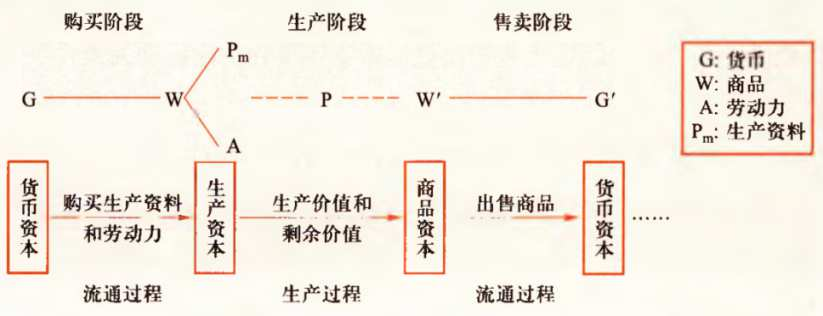
\includegraphics[width=\textwidth]{Pictures/my.png}
\end{figure}
\FloatBarrier

\subsubsection{社会总产品。}
\begin{itemize}
    \item 物质形态：用于生产消费的生产资料、用于生活消费的消费资料。
    \item 价值形态：在产品中的生产资料的转移价值、凝结在产品中的由工人必要劳动时间创造的价值、凝结在产品中的由工人在剩余劳动时间里创造的价值。
\end{itemize}

\subsubsection{资本主义工资。}
\begin{itemize}
    \item 本质：资本主义制度下，工人的工资是劳动力的价值或价格。
    \item 模糊了工人必要劳动和剩余劳动的界限，掩盖了资本主义的剥削关系。
\end{itemize}

\subsubsection{资本主义经济危机。}
\begin{itemize}
    \item 资本主义发展到一定阶段，就会发生以生产过剩为基本特征的经济危机。
    \item 经济危机的抽象的一般的可能性，首先是由货币作为流通手段和支付手段引起的。
    \item 资本主义经济危机爆发的根本原因是资本主义的基本矛盾。
    \item 资本主义经济危机具有周期性，这是由资本主义基本矛盾运动的阶段性决定的。
\end{itemize}

\subsubsection{资本主义国家的职能和本质。}
\begin{itemize}
    \item 职能：以服务于资本主义制度和资产阶级利益为根本内容。
    \item 本质：资产阶级进行阶级统治的工具。
\end{itemize}

\subsubsection{资本主义意识形态的本质。}
\begin{itemize}
    \item 资本主义意识形态是资本主义社会的观念上层建筑，是为资本主义的经济基础服务的，因而是为资本主义国家的政治上层建筑服务的；
    \item 资本主义意识形态是资产阶级的阶级意识的集中体现。
\end{itemize}

\newpage

\section{系统工程}

\subsection{系统工程概述}

\subsubsection{系统。}
\begin{itemize}
    \item 定义：由两个及以上有机联系、相互作用的要素所组成，具有特定功能、结构和环境的整体。
    \item 一般属性：整体性、关联性、环境适应性、目的性、层次性。
\end{itemize}

\subsubsection{系统工程。}
\begin{itemize}
    \item 定义：从总体出发，合理开发、运行和革新一个大规模复杂系统所需思想、理论、方法论、方法与技术的总称。
    \item 研究对象：大规模复杂系统问题。
    \item 理论基础：由一般系统论及其发展、大系统理论、经济控制论、运筹学、管理科学等学科相互渗透、交叉发展而形成的。
\end{itemize}

\subsubsection{系统工程方法的思想及应用要求。}
\begin{itemize}
    \item 系统的观点（前提）；
    \item 总体最优及平衡协调的观点（目的）；
    \item 综合运用方法与技术的观点（手段）；
    \item 问题导向和反馈控制的观点（保障）。
\end{itemize}

\subsubsection{系统工程与传统工程的区别。}
\begin{itemize}
    \item 系统工程一般采用先决定整体框架，后进入内部详细设计的程序；
    \item 系统工程试图通过将构成事物的要素的秩序加以适当配置来提高整体的功能，其核心思想是“综合即创造”；
    \item 系统工程是软科学，其基本特征是人和信息的重要作用、多次反馈和反复协商、科学性与艺术性的二重性及其有机结合等；
    \item 系统工程成为一门综合、横向、通用的科学方法，重要性日益凸显。
\end{itemize}

\subsubsection{系统工程的特点。}
\begin{itemize}
    \item 科学性与艺术性兼容；
    \item 多领域、多学科的理论、方法与技术的集成；
    \item 定性分析与定量分析有机结合；
    \item 需要各有关方面的协作。
\end{itemize}

\subsection{系统工程方法论}

\subsubsection{霍尔三维结构。}
\begin{itemize}
    \item 结构：时间维、逻辑维、知识维或专业维。
    \item 基本思想：强调明确目标，核心内容是最优化，并认为现实问题基本上都可归纳为工程系统问题，应用定量分析手段，求得最优解答。
    \item 特点：
    \begin{itemize}
        \item 研究方法上的整体性（三维）；
        \item 技术应用上的综合性（知识维或专业维）；
        \item 组织管理上的科学性（时间维与逻辑维）；
        \item 系统工程工作的问题导向性（逻辑维）。
    \end{itemize}
\end{itemize}

\subsubsection{切克兰德方法论。}
\begin{itemize}
    \item 基本思想：核心是“比较”与“探寻”，目标是“改善”，强调从“理想”模式与现实状况的比较中探寻改善现状的途径，使决策者满意。
    \item 工作过程：认识问题、根底定义、建立概念模型、比较及探寻、选择、设计与实施、评估与反馈。
\end{itemize}

\subsubsection{霍尔方法论与切克兰德方法论的异同。}
\begin{itemize}
    \item 二者均为系统工程方法论，均以问题为起点，具有相应的逻辑过程；
    \item 霍尔三维结构主要以工程系统为研究对象，而切克兰德方法论更适合对社会经济和经营管理等“软系统”问题进行研究；
    \item 前者的核心内容是优化分析，而后者的核心内容是比较学习；
    \item 前者更多地关注定量分析方法，而后者比较强调定性或定性与定量有机结合的方法。
\end{itemize}

\subsubsection{系统分析。}
\begin{itemize}
    \item 定义：系统分析是运用建模及预测、优化、仿真、评价等技术对系统的各有关方面进行定性与定量相结合的分析，为选择最优或满意的系统方案提供决策依据的分析研究过程。
    \item 要素：问题、目的及目标、方案、模型、评价、决策者。
\end{itemize}

\subsubsection{系统分析的基本过程。}
\begin{figure}[htbp]
    \centering
    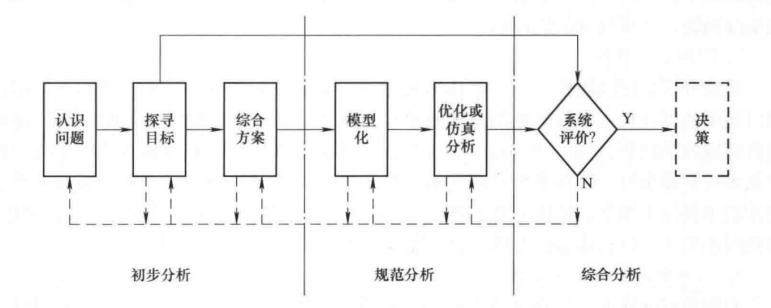
\includegraphics[width=\textwidth]{Pictures/xt1.png}
\end{figure}
\FloatBarrier

\subsubsection{系统分析的主要原则。}
\begin{itemize}
    \item 坚持系统观念；
    \item 坚持问题导向；
    \item 以整体为目标；
    \item 多方案模型分析与选优；
    \item 定量分析与定性分析相结合；
    \item 多次反复进行。
\end{itemize}

\subsubsection{创新分析方法。}
提问法、头脑风暴法、德尔菲法、情景分析法、定性研究方法、数据挖掘方法。

\subsection{系统模型与模型化}

\subsubsection{模型。}
\begin{itemize}
    \item 定义：模型是研究与解决问题的基本框架，可以起到帮助认识系统、模拟系统和优化与改造系统的作用，是对实际系统问题的描述、模仿或抽象。
    \item 特征：
    \begin{itemize}
        \item 是现实世界部分的抽象或模仿；
        \item 是由那些与分析的问题有关的因素构成的；
        \item 表明了有关因素间的相互关系。
    \end{itemize}
    \item 分类：概念模型、符号模型、形象模型、类比模型、仿真模型。
\end{itemize}

\subsubsection{模型化。}
\begin{itemize}
    \item 定义：为描述系统的构成和行为，对实体系统的各种因素进行适当筛选，用一定方式表达系统实体的方法。
    \item 基本方法：分析法、实验法、综合法、老手法、辩证法。
\end{itemize}

\subsubsection{建构模型。}
\begin{itemize}
    \item 一般原则：建立方框图、考虑信息相关性、考虑准确性、考虑结集性。
    \item 基本步骤：
    \begin{itemize}
        \item 明确建模的目的和要求；
        \item 对系统进行一般语言描述；
        \item 弄清楚系统中的主要因素及其相互关系；
        \item 确定模型的结构；
        \item 估计模型的参数；
        \item 实验研究；
        \item 必要修改。
    \end{itemize}
\end{itemize}

\subsubsection{简化模型的方法。}
\begin{itemize}
    \item 减少变量，减去次要变量；
    \item 改变变量性质；
    \item 合并变量；
    \item 改变函数关系；
    \item 改变约束条件。
\end{itemize}

\subsubsection{结构分析。}
\begin{itemize}
    \item 结构：组成系统诸要素之间相互关联的方式。
    \item 结构模型：定性表示系统构成要素以及它们之间存在着的本质上相互依赖、相互制约和关联情况的模型。
    \item 结构模型化：建立系统结构模型的过程。
    \item 结构分析：实现系统结构模型化并加以解释的过程。
\end{itemize}

\subsubsection{系统结构的矩阵表达。}
\begin{itemize}
    \item 邻接矩阵：表示系统要素间基本二元关系或直接联系情况的方阵。
    \item 可达矩阵：表示系统要素之间任意次传递性二元关系，或有向图上两个节点之间通过任意长的路径可以到达情况的方阵。
    \item 缩减矩阵：在可达矩阵中，将具有强连接关系的一组要素看作一个要素，保留其中某个代表要素，删除其余要素的及其行和列，得到该可达矩阵的缩减矩阵。
    \item 骨架矩阵：实现某一可达矩阵的、具有最小二元关系个数的邻接矩阵。
\end{itemize}

\subsubsection{解释结构模型。}
\begin{itemize}
    \item 基本思想：通过有关创新分析方法，提取问题的构成要素，利用有向图、矩阵等工具和计算机技术，对要素及其相互关系等信息进行处理，最后用文字加以解释说明，明确问题的层次和整体结构，提高对问题的认识和理解程度。
    \item 核心内容：通过对可达矩阵的处理，建立系统问题的递阶结构模型。
    \item 特点：不需高深的数学知识、模型直观且有启发性、可吸收各种有关人员参加。
\end{itemize}

\subsubsection{区域划分。}
\begin{itemize}
    \item 可达集$R(S_i)$：从该元素能到达其它元素的那些元素集合。
    \item 先行集$A(S_i)$：能从其它元素到达该元素的那些元素集合。
    \item 共同集$C(S_i)$：可达集和先行集中共同元素集合。
    \item 起始集$B(S)$：系统的输入要素，在有向图中只有箭线流出，而无箭线流入。
    \item 终止集$E(S)$：系统的输出要素，在有向图中只有箭线流入，而无箭线流出。
\end{itemize}

\subsubsection{规范方法。}
\begin{figure}[htbp]
    \centering
    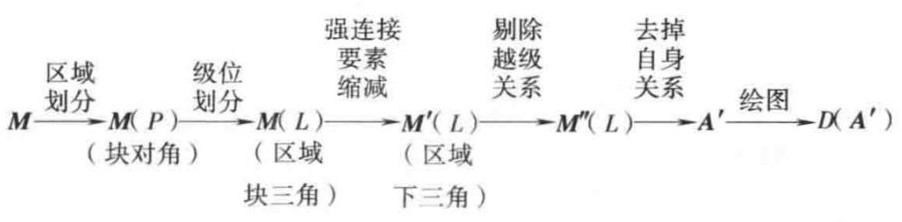
\includegraphics[width=\textwidth]{Pictures/xt2.png}
\end{figure}
\FloatBarrier

\subsubsection{聚类分析。}
按照事物属性的内在联系规律和一定的要求，对事物进行分类研究的方法。

\subsubsection{状态。}
\begin{itemize}
    \item 状态：完全描述$t\geq t_0$时系统行为所需变量的最小集合，该集合构成状态空间。
    \item 状态变量：上述最小变量集合中的每个变量，是描述系统内部动态特性行为的变量。
\end{itemize}

\subsubsection{动态系统。}
\begin{itemize}
    \item 连续动态系统：数学模型是微分方程，刻画系统的动态变量对状态变量的依存关系以及状态变量之间的相互影响。
    \item 离散动态系统：数学模型是差分方程。
\end{itemize}

\subsection{系统仿真及系统动力学方法}

\subsubsection{系统动力学。}
\begin{itemize}
    \item 定义：一种对社会经济问题进行系统分析的方法论和定性与定量相结合的分析方法。
    \item 研究对象：社会（经济）系统。
    \item 结构特点：决策性、自律性、非线性。
    \item 模型特点：
    \begin{itemize}
        \item 多变量；
        \item 定性和定量分析相结合；
        \item 以仿真实验为基本手段和以计算机为工具；
        \item 可处理高阶次、多回路、非线性的时变复杂系统问题。
    \end{itemize}
\end{itemize}

\subsubsection{系统动力学的工作程序。}
\begin{figure}[htbp]
    \centering
    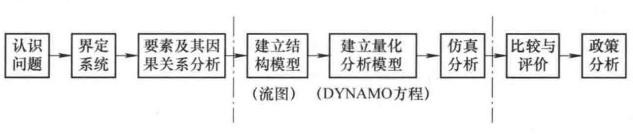
\includegraphics[width=\textwidth]{Pictures/xt3.png}
\end{figure}
\FloatBarrier

\subsubsection{系统动力学的基本原理。}
\begin{itemize}
    \item 原理描述：首先通过对实际系统进行观察，采集有关对象系统状态的信息，随后使用有关信息进行决策，决策的结果是采取行动，行动又作用于实际系统，使系统的状态发生变化，这种变化又为观察者提供新的信息，从而形成系统中的反馈回路。
    \item 基本要素：状态或水准、信息、决策或速率、行动或实物流。
    \item 基本变量：
    \begin{itemize}
        \item 水准变量：系统内活动产生的量，是流的积累形成的，说明系统某个时点状态的变量。
        \item 速率变量：控制流的变量，表示活动进行的状态。
    \end{itemize}
    \item 基本思想：反馈控制。
\end{itemize}

\subsubsection{SD结构模型的建模一般步骤。}
\begin{itemize}
    \item 明确系统边界；
    \item 阐明形成系统结构的反馈回路；
    \item 确定反馈回路中的水准变量和速率变量；
    \item 阐明速率变量的子结构或完善、形成各个决策函数。
\end{itemize}

\subsection{系统评价方法}

\subsubsection{系统评价。}
\begin{itemize}
    \item 定义：对系统方案满足系统目标程度的综合分析及判定。
    \item 系统评价问题要素：评价对象、评价主体、评价目的、评价时期、评价地点、评价方法、评价结果。
\end{itemize}

\subsubsection{效用。}
某主体对某种利益和损失所独有的感觉及反应。

\subsubsection{系统评价程序。}
\begin{figure}[htbp]
    \centering
    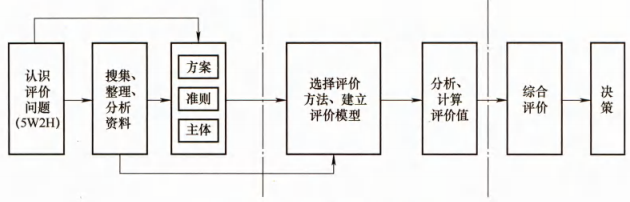
\includegraphics[width=\textwidth]{Pictures/xt5.png}
\end{figure}
\FloatBarrier

\subsubsection{关联矩阵法。}
\begin{itemize}
    \item 定义：用矩阵的形式来表示各替代方案有关评价指标及其重要度与方案关于具体指标的价值评定量之间的关系。
    \item 关键:确定各评价指标的相对重要度（$W_i$）以及关于评价指标的价值评定量（$V_{ij}$），然后计算其综合评价值，即加权和。
    \item 确定权重与价值评定量的方法：逐对比较法和古林法。
\end{itemize}

\subsubsection{层次分析法。}
建立多要素、多层次的评价系统，采用定性与定量有机结合的方法或通过定性信息定量化的途径，使复杂的评价问题明朗化。

\subsubsection{模糊综合评判法。}
\begin{itemize}
    \item 因素集$F$：评价项目或指标的集合。
    \item 评定集$E$：评价等级的集合。
    \item 隶属度$r_{ij}$：多个评价主体对某个评价对象在$f_i$方面做出$e_j$评定的可能性大小。
    \item 隶属度向量$R_i$：评价对象在$f_i$方面的综合评定向量。
    \item 隶属度矩阵$R$：由各评价对象在各评价指标方面的综合评定向量组成的矩阵。
    \item 权重向量$W_F$：评价项目或指标的权重或权系数向量。
\end{itemize}

\subsection{决策分析方法}

\subsubsection{决策。}
\begin{itemize}
    \item 决策：决策是管理的重要职能，是决策者对系统方案所做决定的过程和结果，是决策者的行为和职责。
    \item 管理决策分析：是为帮助决策者在多变的环境条件下进行正确决策而提供的一套推理方法、逻辑步骤和具体技术，以及利用这些方法和技术规范选择满意的行动过程的过程。
\end{itemize}

\subsubsection{决策问题的基本模式。}
\begin{itemize}
    \item $W_{ij}=f(A_i,\theta_j),i=1,2,\ldots,n,j=1,2,\ldots,m$。
    \item $A_i$：决策者的第$i$种策略或第$i$种方案，属于决策变量，是决策者的可控因素。
    \item $\theta_j$：决策者和决策对象（决策问题）所处的第$j$种环境条件或第$j$种自然状态，属于状态变量，是决策者不可控制的因素。
    \item $W_{ij}$：决策者在第$j$种状态下选择第$i$种方案的结果，是决策问题的价值函数值一般叫益损值、效用值。
\end{itemize}

\subsubsection{决策问题的类型。}
\begin{itemize}
    \item 确定型决策：存在确定的自然状态。
    \item 风险型决策：存在两个及以上不以决策者主观意志为转移的自然状态，但决策者或分析人员根据过去的经验和科学理论等可预先估算出自然状态的概率值。
    \item 不确定型决策：自然状态不确定，且其出现的概率不可知。
    \item 对抗性决策：$W_{ij}=f(A_i, B_j),i=1,2,\ldots,n, j=1,2,\ldots,m$，其中$A_i$是决策者的策略集，$B_j$是竞争对手的策略集。
    \item 多目标决策：通常要同时考虑多个目标的决策。
\end{itemize}

\subsubsection{信息价值。}
\begin{itemize}
    \item 完全信息：据此可以得到完全肯定的自然状态信息，有助于正确决策，使决策结果获得较大的收益。
    \item 抽样信息：通过抽样获得的信息，用统计方法推断自然状态出现的概率，据此来选择行动的方案。
    \item 信息价值：获取信息时益损值的期望$-$不获取信息时益损值的期望$-$信息本身成本代价。
\end{itemize}

\subsubsection{冲突分析。}
\begin{itemize}
    \item 冲突分析：国外在经典对策论和偏对策理论基础上发展起来的一种对冲突行为进行正规分析的决策分析方法。
    \item 对策：决策者在某种竞争场合下做出的决策，是一种人为的不确定型决策。
\end{itemize}

\subsubsection{冲突分析方法的特点。}
\begin{itemize}
    \item 能最大限度地利用信息，尤其对许多难以定量分析的问题，因而较适于解决工程系统中考虑社会因素影响时的决策问题和社会系统中的多人决策问题；
    \item 具有严谨的数学和逻辑学基础，是在一般对策论基础上发展起来的偏对策理论的实际应用；
    \item 既能进行冲突事态的结果预测，又能进行事态的过程描述和评估，从而可为决策者提供多方面有价值的决策信息，并可进行政策和决策行为的分析；
    \item 分析方法在使用中几乎不需要任何数学理论和复杂的数学方法，很容易被理解和掌握，主要分析过程还可用计算机，通过人-机对话解决，因而具有很强的实用性；
    \item 用结局的优先序代替了效用值，并认为对结局进行比较判断时可无传递性，从而在实际应用中避开了经典对策论关于效用值和传递性假设等障碍。
\end{itemize}

\subsubsection{冲突分析的一般程序。}
\begin{figure}[htbp]
    \centering
    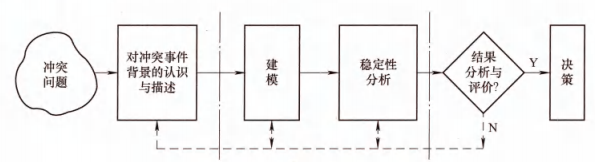
\includegraphics[width=\textwidth]{Pictures/xt8.png}
\end{figure}
\FloatBarrier

\subsubsection{冲突分析的基本要素。}
时间点、局中人、选择或行动、结局、优先序或优先向量。

\subsubsection{稳定性分析。}
\begin{itemize}
    \item 单方面改进（UI）：某一局中人不改变其策略，而另一局中人单方面改变其策略使自己的处境更好则形成单方面改进。
    \item 合理性稳定：对于局中人$A$考虑结局$q$，如果不存在UI，则对于$A$，$q$是合理稳定的结局，记作$r$。
    \item 连续处罚性稳定结局：对于局中人$A$考虑结局$q$，如果存在UI结局$q'$，而$q'$对于局中人$B$也存在UI结局$q''$，但$q''$对于$A$不比$q$更优，称$q$的UI结局$q'$存在一个连续性处罚。对于$A$的结局$q$的全部UI结局都存在连续性处罚，则称对于$A$，$q$为连续处罚性稳定结局，记作$s$。
    \item 非稳定结局：对于局中人$A$，考虑结局$q$，如果存在UI但又不是$s$，则称对于$A$，$q$是非稳定结局，记作$u$。
    \item 同时处罚性稳定结局：冲突双方均为不稳定结局时，通过合成的结局，对局中人而言，不比该结局更优，则称该结局为同时处罚性稳定结局，记作$\cancel{u}$。对局中人而言，某结局全部UI都存在同时性处罚，则该结局才算做同时性处罚结局。
    \item 全局平稳结局：对于每个局中人都属于$(r,s,\cancel{u})$的结局为全局平稳结局，记作$E$。
\end{itemize}

\newpage

\section*{写在后面}
\addcontentsline{toc}{section}{写在后面}

真的要写这个结尾吗？这玩意感觉整理得也不好，就先这样吧。笔者听说明年将迎来新一轮的思政课大改革，什么毛概史纲二合一，好像今年5+3那边已经开始试点了来着，那很有生活了。这个资料反正终究会成为时代的眼泪，当个纪念也好。

本资料的封面为word排版制作，目录和正文部分则使用latex自创模板排版制作。在此感谢这两款软件的支持。

如有任何问题，请加qq：1743495223与笔者联系，互相交流学习或者扩列也行。

祝各位学业有成！

\rightline{杨承轩}

\rightline{丙午，五月十一，碑林}
\end{document}